\documentclass{article}
\usepackage[a4paper,top=1.5cm,bottom=1.5cm,left=2cm,right=2cm,marginparwidth=1.75cm]{geometry}
\usepackage{graphicx}
\usepackage{setspace}
\usepackage{ctex}
\usepackage{enumitem}
\usepackage{tabularx}
\usepackage{booktabs}
\usepackage{array}
\usepackage{float}

\begin{document}

\begin{center}
    \vspace*{3cm} % 控制顶部空白
    {\Huge 《数据库系统原理》大作业 \\[1cm]}
    {\LARGE 系统设计报告 \\[5cm]}
\end{center}

\begin{center}
    {\Large 题目名称:航医通} \\[4cm]
\end{center}

\begin{center}
    \begin{tabular}{ll}
        {\Large 学号及姓名:} & {\Large \underline{22371056 孟烜宇(组长)}} \\[0.5cm]
        & {\Large \underline{22373040 余欣实}} \\[0.5cm]
        & {\Large \underline{22371328 曹玮琳}} \\[3cm]
    \end{tabular}
\end{center}

\begin{center}
    {\Large 2024\hspace{0.35cm} 年 \hspace{0.35cm} 10\hspace{0.35cm} 月 \hspace{0.35cm} 4\hspace{0.35cm} 日}
\end{center}

\newpage

\begin{center}
    \vspace*{3cm}
    \LARGE 组内同学承担任务说明
\end{center}

\vspace{2.5cm}

\begin{center}
\renewcommand{\arraystretch}{3} % 调整行高
\setlength{\tabcolsep}{10pt} % 调整列间距
\small % 调整字体大小
\begin{tabular}{|c|p{2cm}|p{2cm}|p{2cm}|c|}
    \hline
    \textbf{学生姓名} & \multicolumn{3}{c|}{\textbf{工作内容}} & \textbf{工作量占比} \\ 
    \cline{2-4}
     & \textbf{子任务 1:系统功能设计与数据库设计} & \textbf{子任务 2:系统服务器端开发} & \textbf{子任务 3:系统客户端开发} & \textbf{(组内同学总和为 1)} \\
    \hline
    孟烜宇& & & & \\
    \hline
    余欣实& & & & \\
    \hline
    曹玮琳& & & & \\
    \hline
\end{tabular}
\end{center}

\newpage

\tableofcontents

\newpage

\section{需求分析}
\subsection{需求描述}
\subsubsection{背景调研}

社会发展不停歇,人们对于医疗服务的需求也在不断增加。在这种情况下,医疗服务的质量和效率也成为了人们关注的焦点。
与此同时,大学生作为国家的希望与未来,其身体健康状况引起了社会的广泛关注。但是,大学生的健康却不容乐观。诸如“脆皮大学生”等问题愈演愈烈,睡眠质量不足、饮食不规律、容易受伤等问题困扰着许多大学生。
大学如何担起培养社会主义现代化强国的建设者和接班人的伟大使命?
高校医疗健康体系如何在中华民族伟大复兴战略全局和世界百年未有之大变局中,顺应潮流把握机遇,面临挑战?
为祖国培养“健康工作七十年的红色工程师”的北京航空航天大学,应当以怎样的技术和平台来保证学生的医疗健康呢?
这些问题值得我们深思。

首先,必须认识到校园医疗服务的多元性,涵盖从日常健康管理到突发疾病的应急处理。
这种多元性意味着校园医疗服务不仅要提供基础的医疗诊断和治疗,还需要针对不同疾病类型和健康问题提供个性化的解决方案,以满足学生的各种需求。通过全面的服务体系,能够更有效地应对学生在学习和生活中可能遇到的健康挑战。

其次,通过构建一个集成化的医疗服务平台,不仅能够提升学生的就医体验,还能为学校的整体健康教育提供数据支持和决策依据。
该平台可以集中管理学生的健康档案、就医记录和预约信息,使得医疗服务更加高效和便捷。同时,汇总的数据可以帮助学校分析学生的健康趋势,识别常见健康问题,从而制定更具针对性的健康教育方案和预防措施,以提高整体校园健康水平。

但是,北京航空航天大学目前缺少这么一个完善的医疗服务网络平台。学生在体检、就医等过程中程序繁琐,信息不对称,导致就医效率低下,学校也无法全面了解学生的健康状况。

因此,本团队希望开发一个功能强大且集成,数据安全的医疗服务平台,以提升学生的就医体验,提高学校的医疗服务水平。
这就是航医通开发的初衷。

\subsubsection{用户画像}
校园医疗服务平台的主要用户有以下几类:

\begin{itemize}[itemsep=0.01em]
    \item 在读学生与教职工
    \item 医护人员
    \item 管理人员
\end{itemize}

\begin{figure}[h]
    \centering
    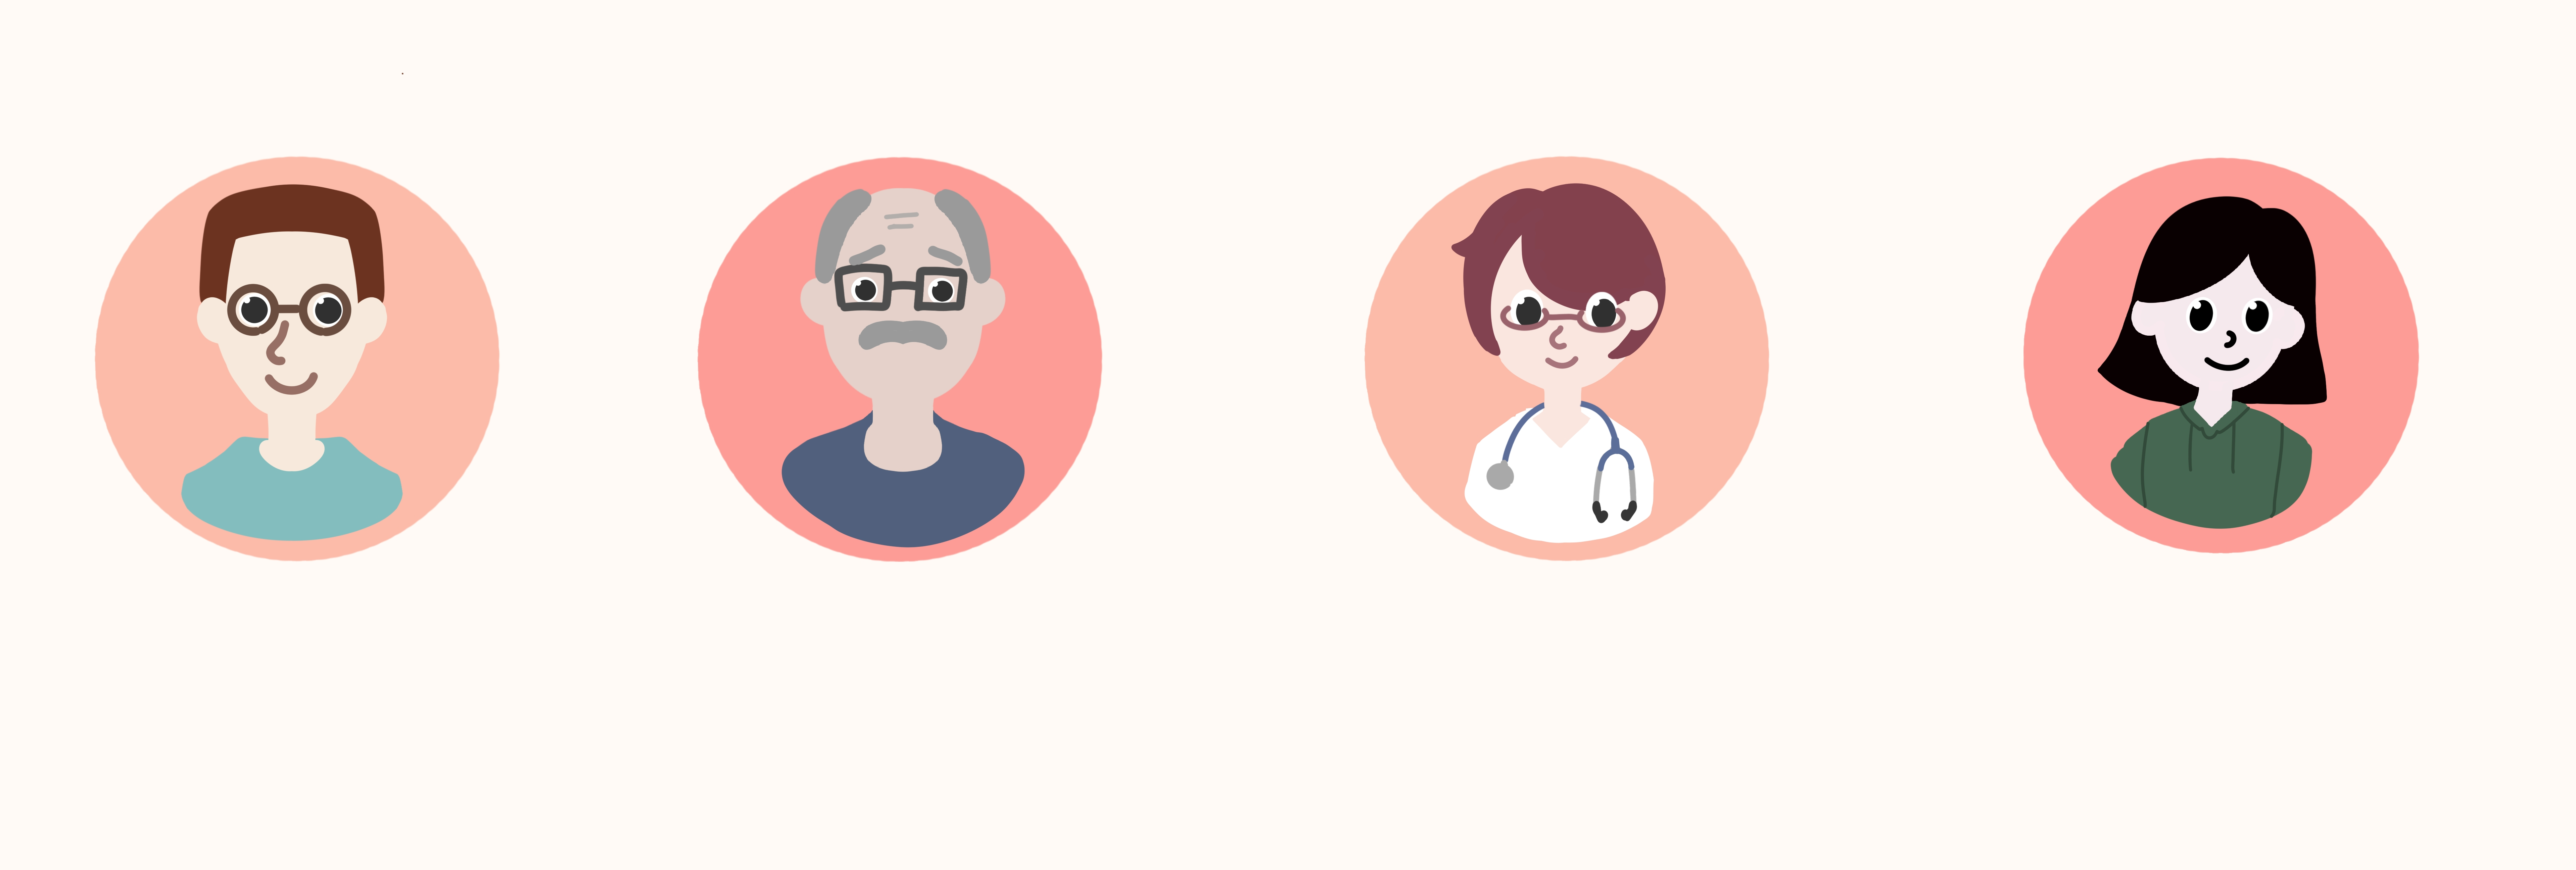
\includegraphics[width=0.8\textwidth]{images/user.jpg}
    \caption{用户画像}
\end{figure}

\subsubsection{需求分析}

经过上述背景调研和用户画像的分析,我们可以总结出需求如下:
\vspace{0.5cm}

对于每一位在读学生以及教职工,我们希望能够提供以下服务:
\begin{enumerate}[itemsep=0.01em]
    \item 拥有在线上查看医生排班并为自己\textbf{预约挂号}权限,能够选择合适时间段就诊。
    \item 能够查看自己的排队信息,\textbf{候诊查询}。
    \item 
    能够线上进行\textbf{在线缴费},包括挂号费、药费等。
    \item 对于每年的体检,能够在线上选择体检时间和项目,\textbf{预约体检}。
    \item 可以对于就诊经历进行评价,提供\textbf{医生评价}功能。
    \item 能够查看自己的\textbf{健康档案},包括体检记录、病历、就诊记录、处方等。
    \item 能够接受相关\textbf{通知提醒},如体检提醒、就诊提醒等。
    \item 定期接受\textbf{健康讲座},提供健康教育。
\end{enumerate}

除此之外,对于教职工,我们还希望能够提供为他们的家属进行\textbf{预约挂号}、\textbf{候诊查询}、\textbf{家属健康档案}的服务。

\vspace{0.5cm}
对于医护人员,我们希望能够提供以下服务:
\begin{enumerate}[itemsep=0.01em]
    \item 能够查看自己的\textbf{排班信息}。
    \item 可以查看预约记录,\textbf{预约查询}。
    \item 可以查看排队信息,\textbf{候诊查询}。
    \item 可以查看\textbf{患者信息},包括病历、就诊记录、处方等。
    \item 可以查看\textbf{患者评价},并进行回复。
    \item 能够接受相关\textbf{通知提醒},如排班提醒、患者评价提醒等。
    \item 能够创建或者更新\textbf{患者病历}。
    \item 可以开具处方并记录药品信息,\textbf{处方管理}。
\end{enumerate}

\vspace{0.5cm}
对于管理人员,我们希望能够提供以下服务:
\begin{enumerate}[itemsep=0.01em]
    \item 能够查看\textbf{医疗数据分析},包括患者病历统计、疾病统计等。
    \item 可以查看并管理\textbf{医疗服务评价}。
    \item 能够进行\textbf{医疗排班},添加、修改或删除医生的排班信息。
    \item 可以管理药品信息和库存,\textbf{药品管理}。
    \item 查看和管理预约记录,\textbf{预约管理}。
\end{enumerate}

\vspace{0.5cm}
另外对于\textbf{数据库管理员}:
\begin{enumerate}[itemsep=0.01em]
    \item 具有管理用户的权限,可以检索,修改,增加,删除所有的用户信息。
    \item 具有管理预约的权限,可以检索,修改,增加,删除所有的预约信息。
    \item 具有管理药品、处方、病历等信息的权限,可以检索,修改,增加,删除所有的医药信息。
\end{enumerate}

\subsection{数据字典}

\subsubsection{用户管理部分}

\begin{table}[H]
    \centering
    \begin{tabularx}{\textwidth}{|p{2.2cm}|p{3.2cm}|p{4.8cm}|p{5cm}|}
    \toprule
    \textbf{属性名} & \textbf{字段名} & \textbf{数据类型} & \textbf{约束}\\ \midrule
    学工号 & id & char(8) & 主键 \\ \midrule
    密码 & password & varchar(25) & 非空 \\ \midrule
    姓名 & name & varchar(15) & 非空 \\ \midrule
    性别 & gender & char(1) & 非空 \\ \midrule
    出生日期 & birth & date & 非空 \\ \midrule
    身份证号 & id\_number & varchar(18) & 非空 \\ \midrule
    用户类型 & user\_type & char(1) & 非空 \\ \midrule
    手机号 & phone & varchar(11) & 非空 \\ \bottomrule
    \end{tabularx}
    \caption{用户数据字典}
    \label{tab:student_user}
\end{table}

\begin{table}[H]
    \centering
    \begin{tabularx}{\textwidth}{|p{2.2cm}|p{3.2cm}|p{4.8cm}|p{5cm}|}
    \toprule
    \textbf{属性名} & \textbf{字段名} & \textbf{数据类型} & \textbf{约束} \\ \midrule
    医工号 & staff\_id & char(5) & 主键 \\ \midrule
    密码 & password & varchar(25) & 非空 \\ \midrule
    姓名 & name & varchar(15) & 非空 \\ \midrule
    性别 & gender & char(1) & 非空 \\ \midrule
    职称 & title & varchar(10) & 非空 \\ \midrule
    图片号 & image\_id & varchar(10) &  \\ \midrule
    介绍 & introduction & text & 非空 \\ \bottomrule
    \end{tabularx}
    \caption{医师用户数据字典}
    \label{tab:doctor_user}
\end{table}

\begin{table}[H]
    \centering
    \begin{tabularx}{\textwidth}{|p{2.2cm}|p{3.2cm}|p{4.8cm}|p{5cm}|}
    \toprule
    \textbf{属性名} & \textbf{字段名} & \textbf{数据类型} & \textbf{约束} \\ \midrule
    管理员号 & admin\_id & char(3) & 主键 \\ \midrule
    姓名 & name & varchar(15) & 非空 \\ \midrule
    密码 & password & varchar(25) & 非空 \\ \bottomrule
    \end{tabularx}
    \caption{管理员数据字典}
    \label{tab:admin_user}
\end{table}

\begin{table}[H]
    \centering
    \begin{tabularx}{\textwidth}{|p{2.2cm}|p{3.2cm}|p{4.8cm}|p{5cm}|}
    \toprule
    \textbf{属性名} & \textbf{字段名} & \textbf{数据类型} & \textbf{约束} \\ \midrule
    家属号 & family\_id & varchar(2) & 主键 \\ \midrule
    学工号 & id & char(8) & 主键 \\ \midrule
    关系 & relationship & varchar(10) & 非空 \\ \bottomrule
    姓名 & name & varchar(15) & 非空 \\ \midrule
    性别 & gender & char(1) & 非空 \\ \midrule
    出生日期 & birth & date & 非空 \\ \midrule
    身份证号 & id\_number & varchar(18) & 非空 \\ \bottomrule
    \end{tabularx}
    \caption{家属数据字典}
    \label{tab:family_user}
\end{table}

\subsubsection{医疗系统部分}

\begin{table}[H]
    \centering
    \begin{tabularx}{\textwidth}{|p{2.2cm}|p{3.2cm}|p{4.8cm}|p{5cm}|}
    \toprule
    \textbf{属性名} & \textbf{字段名} & \textbf{数据类型} & \textbf{约束} \\ \midrule
    科室号 & department\_id & char(3) & 主键 \\ \midrule
    科室名称 & department\_name & varchar(10) & 非空 \\ \bottomrule
    \end{tabularx}
    \caption{科室数据字典}
    \label{tab:department}
\end{table}

\begin{table}[H]
    \centering
    \begin{tabularx}{\textwidth}{|p{2.2cm}|p{3.2cm}|p{4.8cm}|p{5cm}|}
    \toprule
    \textbf{属性名} & \textbf{字段名} & \textbf{数据类型} & \textbf{约束} \\ \midrule
    排班号 & schedule\_id & char(8) & 主键 \\ \midrule
    医工号 & staff\_id & char(5) & 非空 \\ \midrule
    科室号 & department\_id & char(3) & 非空 \\ \midrule
    排班时间 & schedule\_time & datetime & 非空 \\
    \bottomrule
    \end{tabularx}
    \caption{排班数据字典}
    \label{tab:schedule}
\end{table}

\begin{table}[H]
    \centering
    \begin{tabularx}{\textwidth}{|p{2.2cm}|p{3.2cm}|p{4.8cm}|p{5cm}|}
    \toprule
    \textbf{属性名} & \textbf{字段名} & \textbf{数据类型} & \textbf{约束} \\ \midrule
    药房号 & pharmacy\_id & varchar(2) & 主键 \\ \midrule
    药房名称 & pharmacy\_name & varchar(10) & 非空 \\ \bottomrule
    \end{tabularx}
    \caption{药房数据字典}
    \label{tab:pharmacy}
\end{table}

\begin{table}[H]
    \centering
    \begin{tabularx}{\textwidth}{|p{2.2cm}|p{3.2cm}|p{4.8cm}|p{5cm}|}
    \toprule
    \textbf{属性名} & \textbf{字段名} & \textbf{数据类型} & \textbf{约束} \\ \midrule
    药品号 & drug\_id & varchar(9) & 主键 \\ \midrule
    药品名称 & drug\_name & varchar(20) & 非空 \\ \midrule
    药品价格 & price & float & 非空 \\ \bottomrule
    \end{tabularx}
    \caption{药品数据字典}
    \label{tab:drug}
\end{table}

\begin{table}[H]
    \centering
    \begin{tabularx}{\textwidth}{|p{2.2cm}|p{3.2cm}|p{4.8cm}|p{5cm}|}
    \toprule
    \textbf{属性名} & \textbf{字段名} & \textbf{数据类型} & \textbf{约束} \\ \midrule
    药品号 & drug\_id & varchar(9) & 主键 \\ \midrule
    药品数量 & drug\_amount & int & 非空 \\ \midrule
    药房号 & pharmacy\_id & varchar(2) & 主键 \\ \bottomrule
    \end{tabularx}
    \caption{药品库存数据字典}
    \label{tab:drug_storage}
\end{table}

\subsubsection{预约管理部分}

\begin{table}[H]
    \centering
    \begin{tabularx}{\textwidth}{|p{2.2cm}|p{3.2cm}|p{4.8cm}|p{5cm}|}
    \toprule
    \textbf{属性名} & \textbf{字段名} & \textbf{数据类型} & \textbf{约束} \\ \midrule
    体检号 & examination\_id & varchar(8) & 主键 \\ \midrule
    体检项目 & examination & text & 非空 \\ \midrule
    体检日期 & examination\_date & date & 非空 \\ \midrule
    负责医工号 & staff\_id & char(5) & 非空 \\ \bottomrule
    \end{tabularx}
    \caption{体检安排字典}
    \label{tab:examination_arrangement}
\end{table}

\begin{table}[H]
    \centering
    \begin{tabularx}{\textwidth}{|p{2.2cm}|p{3.3cm}|p{4.7cm}|p{5cm}|}
    \toprule
    \textbf{属性名} & \textbf{字段名} & \textbf{数据类型} & \textbf{约束} \\ \midrule
    体检预约号 & exam\_appointment\_id & varchar(8) & 主键 \\ \midrule
    体检号 & examination\_id & varchar(8) & 非空 \\ \midrule
    体检结果 & examination\_result & text &  \\ \midrule
    学工号 & id & char(8) & 非空 \\ \bottomrule
    \end{tabularx}
    \caption{体检信息数据字典}
    \label{tab:examination_appointment}
\end{table}

\begin{table}[H]
    \centering
    \begin{tabularx}{\textwidth}{|p{2.2cm}|p{3.2cm}|p{4.8cm}|p{5cm}|}
    \toprule
    \textbf{属性名} & \textbf{字段名} & \textbf{数据类型} & \textbf{约束} \\ \midrule
    预约号 & appointment\_id & varchar(8) & 主键 \\ \midrule
    患者与预约人关系 & relationship & varchar(10) & 非空 \\ \midrule
    排班号 & schedule\_id & char(8) & 非空 \\ \midrule
    学工号 & id & varchar(8) & 非空 \\ \bottomrule
    \end{tabularx}
    \caption{预约数据字典}
    \label{tab:appointment}
\end{table}

\begin{table}[H]
    \centering
    \begin{tabularx}{\textwidth}{|p{2.2cm}|p{3.2cm}|p{4.8cm}|p{5cm}|}
    \toprule
    \textbf{属性名} & \textbf{字段名} & \textbf{数据类型} & \textbf{约束} \\ \midrule
    诊断号 & diagnosis\_id & varchar(8) & 主键 \\ \midrule
    检查项目 & examination & text & 非空 \\ \midrule
    检查结果 & examination\_result & text & 非空 \\ \midrule
    参考范围 & reference & text & 非空 \\ \midrule
    临床诊断 & clinical\_diagnosis & text & 非空 \\ \midrule
    处方号 & prescription\_id & varchar(8) & 非空 \\ \midrule
    诊断时间 & diagnosis\_time & datetime & 非空 \\ \midrule
    患者身份证号 & id\_number & varchar(18) & 非空 \\ \midrule
    预约号 & appointment\_id & varchar(8) & 非空 \\ \midrule
    医工号 & staff\_id & char(5) & 非空 \\ \bottomrule
    \end{tabularx}
    \caption{诊断数据字典}
    \label{tab:diagnosis}
\end{table}

\subsubsection{药品管理部分}

\begin{table}[H]
    \centering
    \begin{tabularx}{\textwidth}{|p{2.2cm}|p{3.2cm}|p{4.8cm}|p{5cm}|}
    \toprule
    \textbf{属性名} & \textbf{字段名} & \textbf{数据类型} & \textbf{约束} \\ \midrule
    处方号 & prescription\_id & varchar(8) & 主键 \\ \midrule
    诊断号 & diagnosis\_id & varchar(8) & 非空\\ \midrule
    药品号 & drug\_id & varchar(9) & 非空 \\ \midrule
    药品数量 & drug\_amount & int & 非空 \\ \midrule
    用法用量 & usage & text & 非空 \\ \midrule
    注意事项 & precautions & text & 非空 \\ \bottomrule
    \end{tabularx}
    \caption{处方数据字典}
    \label{tab:prescription}
\end{table}

\subsubsection{其他数据元素}

\begin{table}[H]
    \centering
    \begin{tabularx}{\textwidth}{|p{2.2cm}|p{3.2cm}|p{4.8cm}|p{5cm}|}
    \toprule
    \textbf{属性名} & \textbf{字段名} & \textbf{数据类型} & \textbf{约束} \\ \midrule
    通知号 & notification\_id & varchar(8) & 主键 \\ \midrule
    通知内容 & notification & text & 非空 \\ \midrule
    通知时间 & notification\_time & datetime & 非空 \\ \midrule
    接收人学工号 & staff\_id & varchar(8) & 非空 \\ \bottomrule
    \end{tabularx}
    \caption{通知数据字典}
    \label{tab:notification}   
\end{table}

\begin{table}[H]
    \centering
    \begin{tabularx}{\textwidth}{|p{2.2cm}|p{3.2cm}|p{4.8cm}|p{5cm}|}
    \toprule
    \textbf{属性名} & \textbf{字段名} & \textbf{数据类型} & \textbf{约束} \\ \midrule
    评价号 & evaluation\_id & varchar(8) & 主键 \\ \midrule
    评价内容 & evaluation & text & 非空 \\ \midrule
    评价时间 & evaluation\_time & datetime & 非空 \\ \midrule
    评价人学工号 & id & varchar(8) & 非空 \\ \midrule
    被评价人医工号 & staff\_id & char(5) & 非空 \\ \bottomrule
    \end{tabularx}
    \caption{评价数据字典}
    \label{tab:evaluation}
\end{table}

\begin{table}[H]
    \centering
    \begin{tabularx}{\textwidth}{|p{2.2cm}|p{3.2cm}|p{4.8cm}|p{5cm}|}
    \toprule
    \textbf{属性名} & \textbf{字段名} & \textbf{数据类型} & \textbf{约束} \\ \midrule
    图片号 & image\_id & varchar(10) & 主键 \\ \midrule
    存储路径 & image\_path & varchar(255) & 非空 \\ \midrule
    评价号 & evaluation\_id & varchar(8) &  \\ \midrule
    通知号 & notification\_id & varchar(8) &  \\ \midrule
    药品号 & drug\_id & varchar(9) &  \\ \bottomrule
    \end{tabularx}
    \caption{图片数据字典}
    \label{tab:image}
\end{table}


\subsection{数据流图}

\subsubsection{顶层数据流图}

\begin{figure}[H]
    \centering
    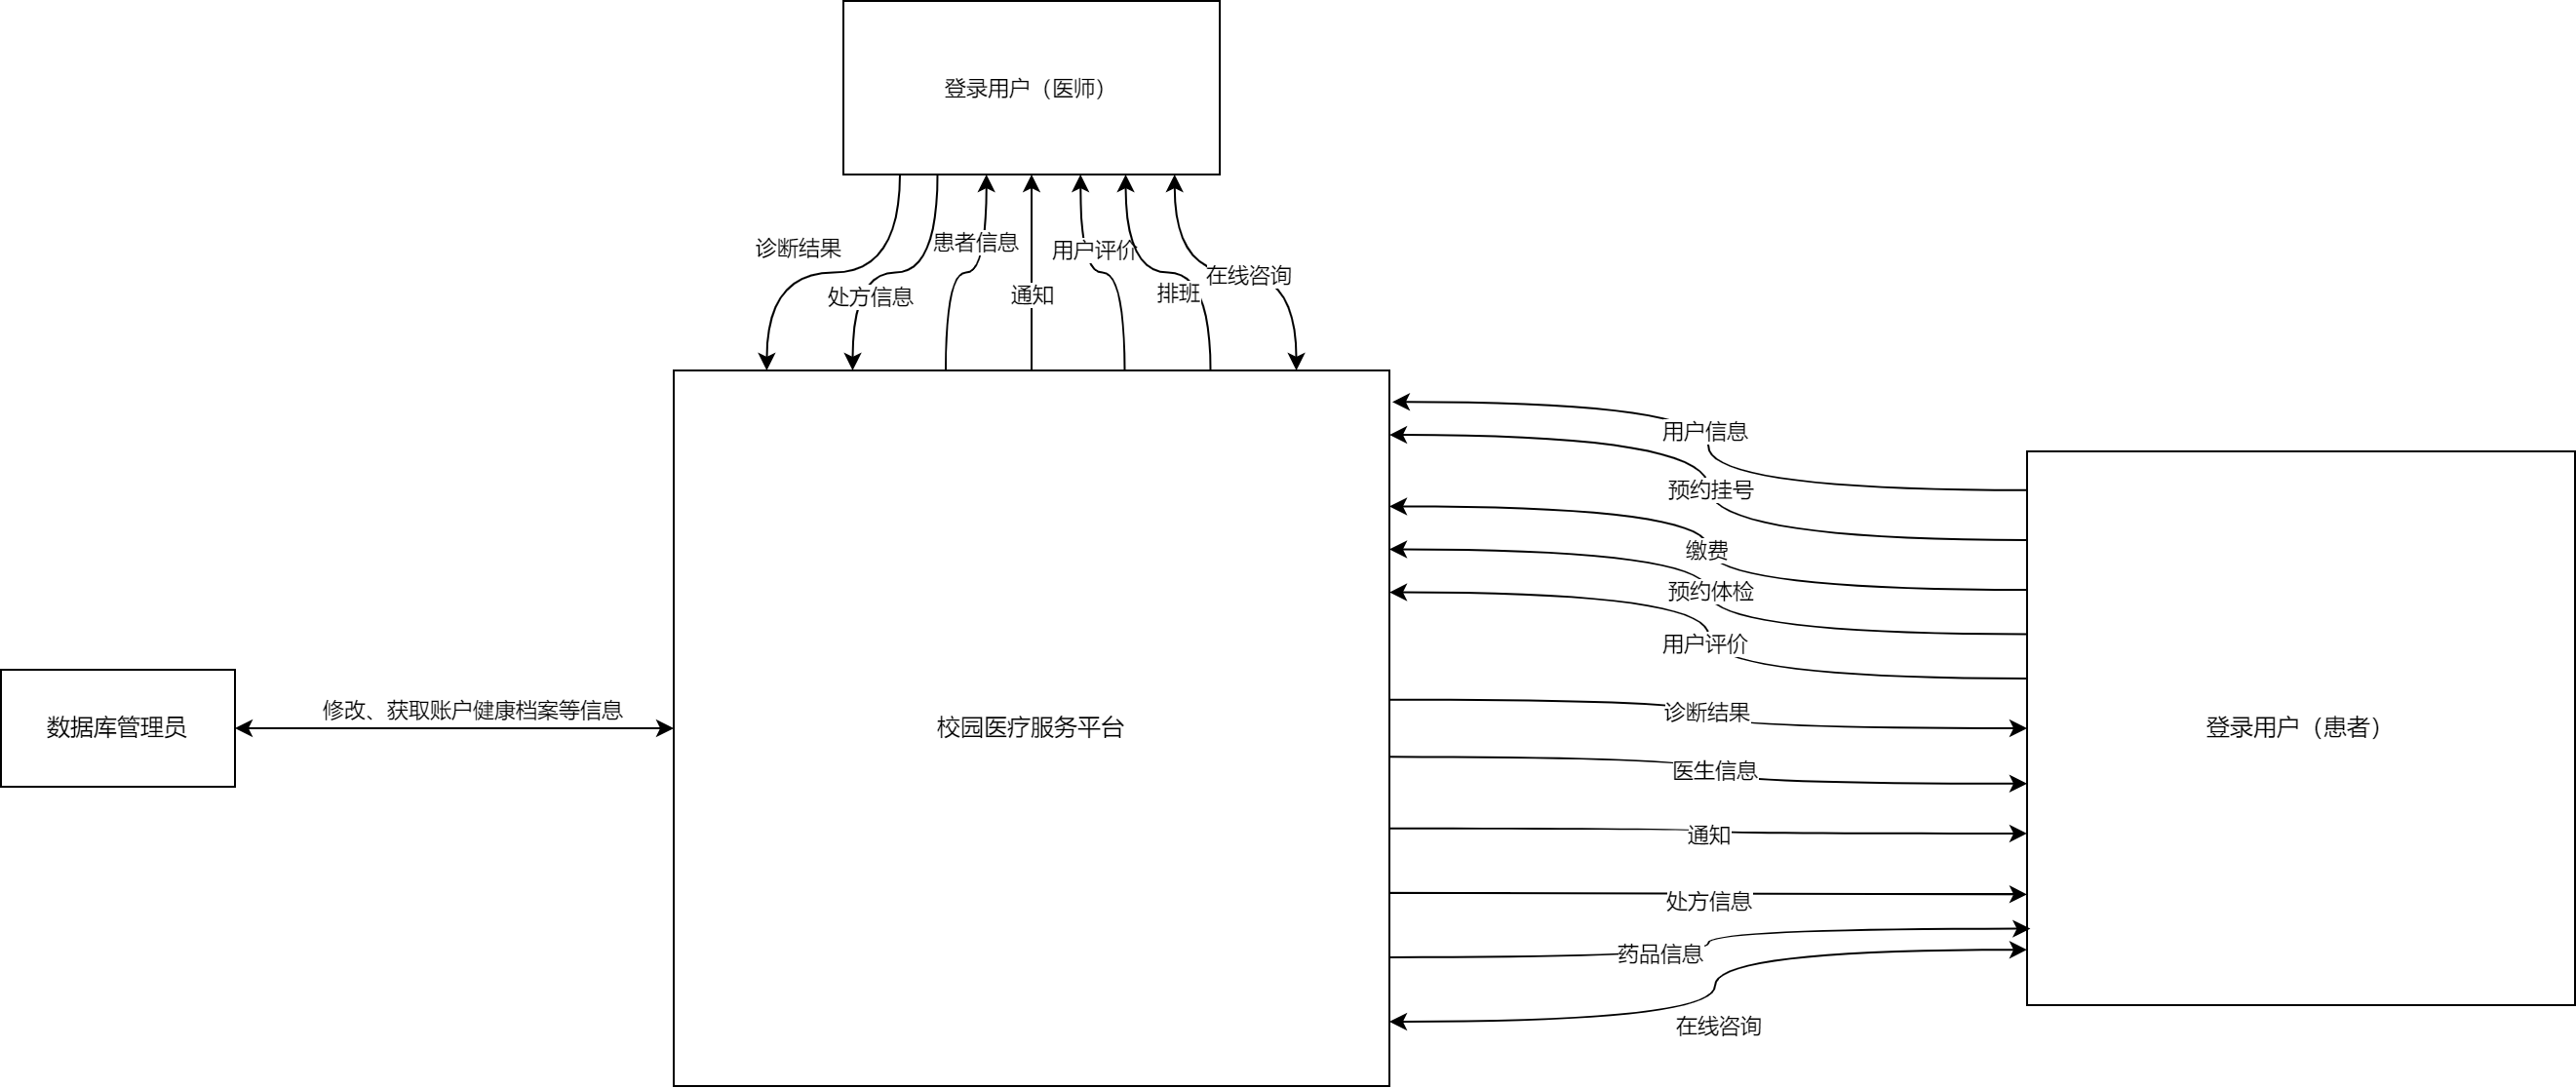
\includegraphics[width=0.8\textwidth]{images/all_dataflow.png}
    \caption{顶层数据流图}
\end{figure}

\subsubsection{层数据流图}

\paragraph{用户系统数据流图}

用户登录时,前端会将登陆类型和账号密码发送给后端,后端会根据账号密码查询数据库,返回用户信息,用户信息会一直保存在前端,直到用户退出登录。

用户修改个人信息或者修改医院用户信息时,前端会将修改后的信息发送给后端,后端会根据用户的学工号查询数据库,修改用户信息。

\begin{figure}[H]
    \centering
    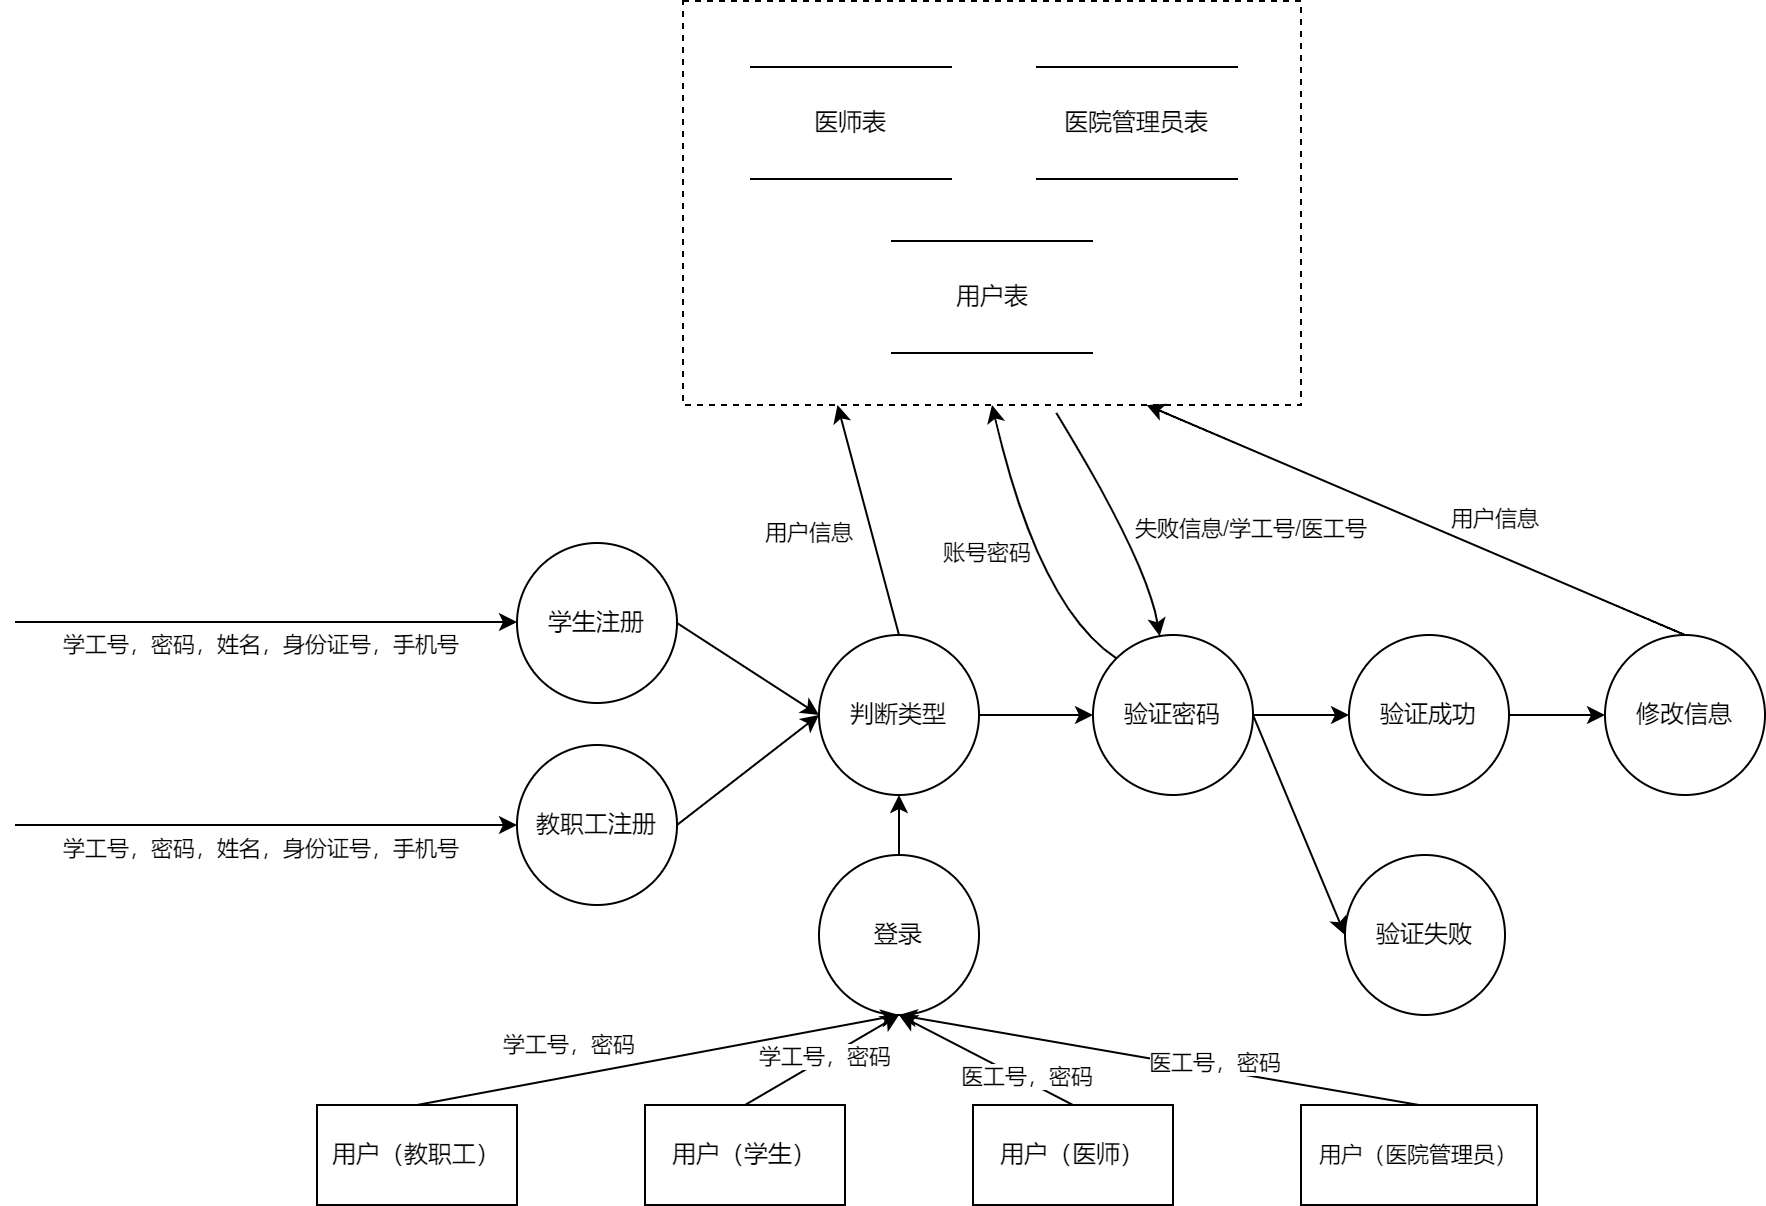
\includegraphics[width=0.8\textwidth]{images/user_dataflow.png}
    \caption{用户系统数据流图}
\end{figure}

\paragraph{医院管理数据流图}

关于医院的管理任务,医院管理员在登陆后,可以查看和更改医院的排班信息,可以查看和更改(比如进药)医院的药品信息,可以录入和更改医院的医师信息,
可以查看和更改(比如因排班调整导致的预约信息的变换)医院的预约信息,可以查看和更改医院的评价信息,可以查看通知和发布通知给指定人员。

\begin{figure}[H]
    \centering
    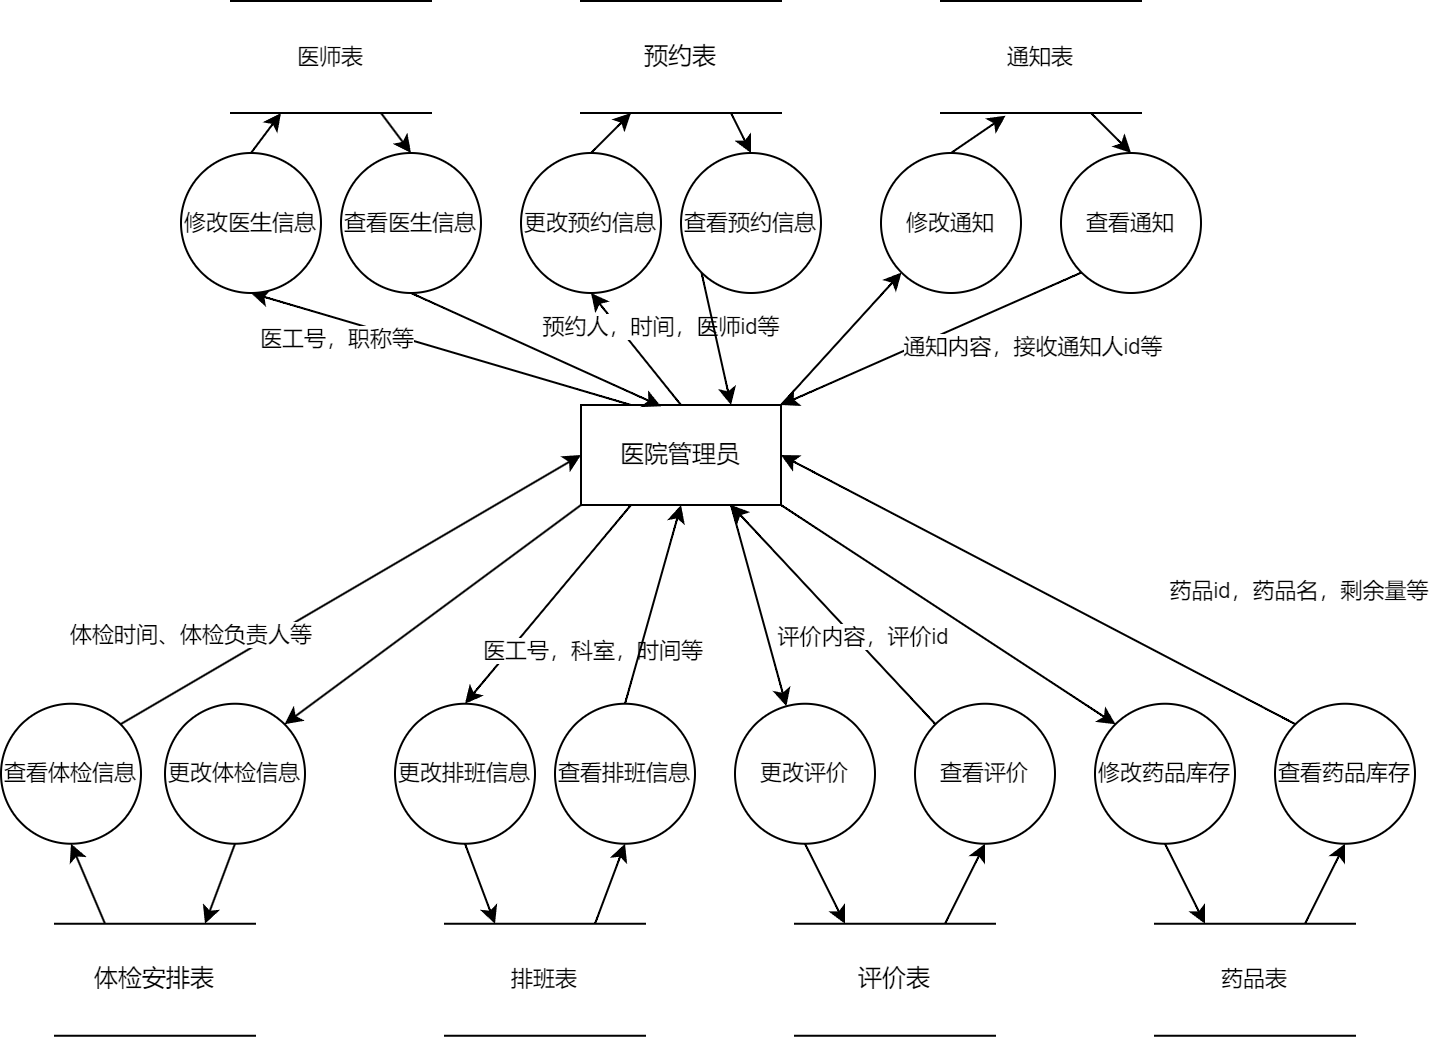
\includegraphics[width=0.8\textwidth]{images/doctorAdmin_dataflow.png}
    \caption{医院管理数据流图}
\end{figure}

\paragraph{预约功能数据流图}

用户在登录后,可以查看医生的排班信息,可以选择预约时间,可以查看自己的预约信息,可以取消预约;医生在登录后,可以查看自己的排班信息和相应的预约信息。

而对于体检,用户在登录后,可以查看体检项目,可以选择体检时间,可以查看自己的体检信息。

\begin{figure}[H]
    \centering
    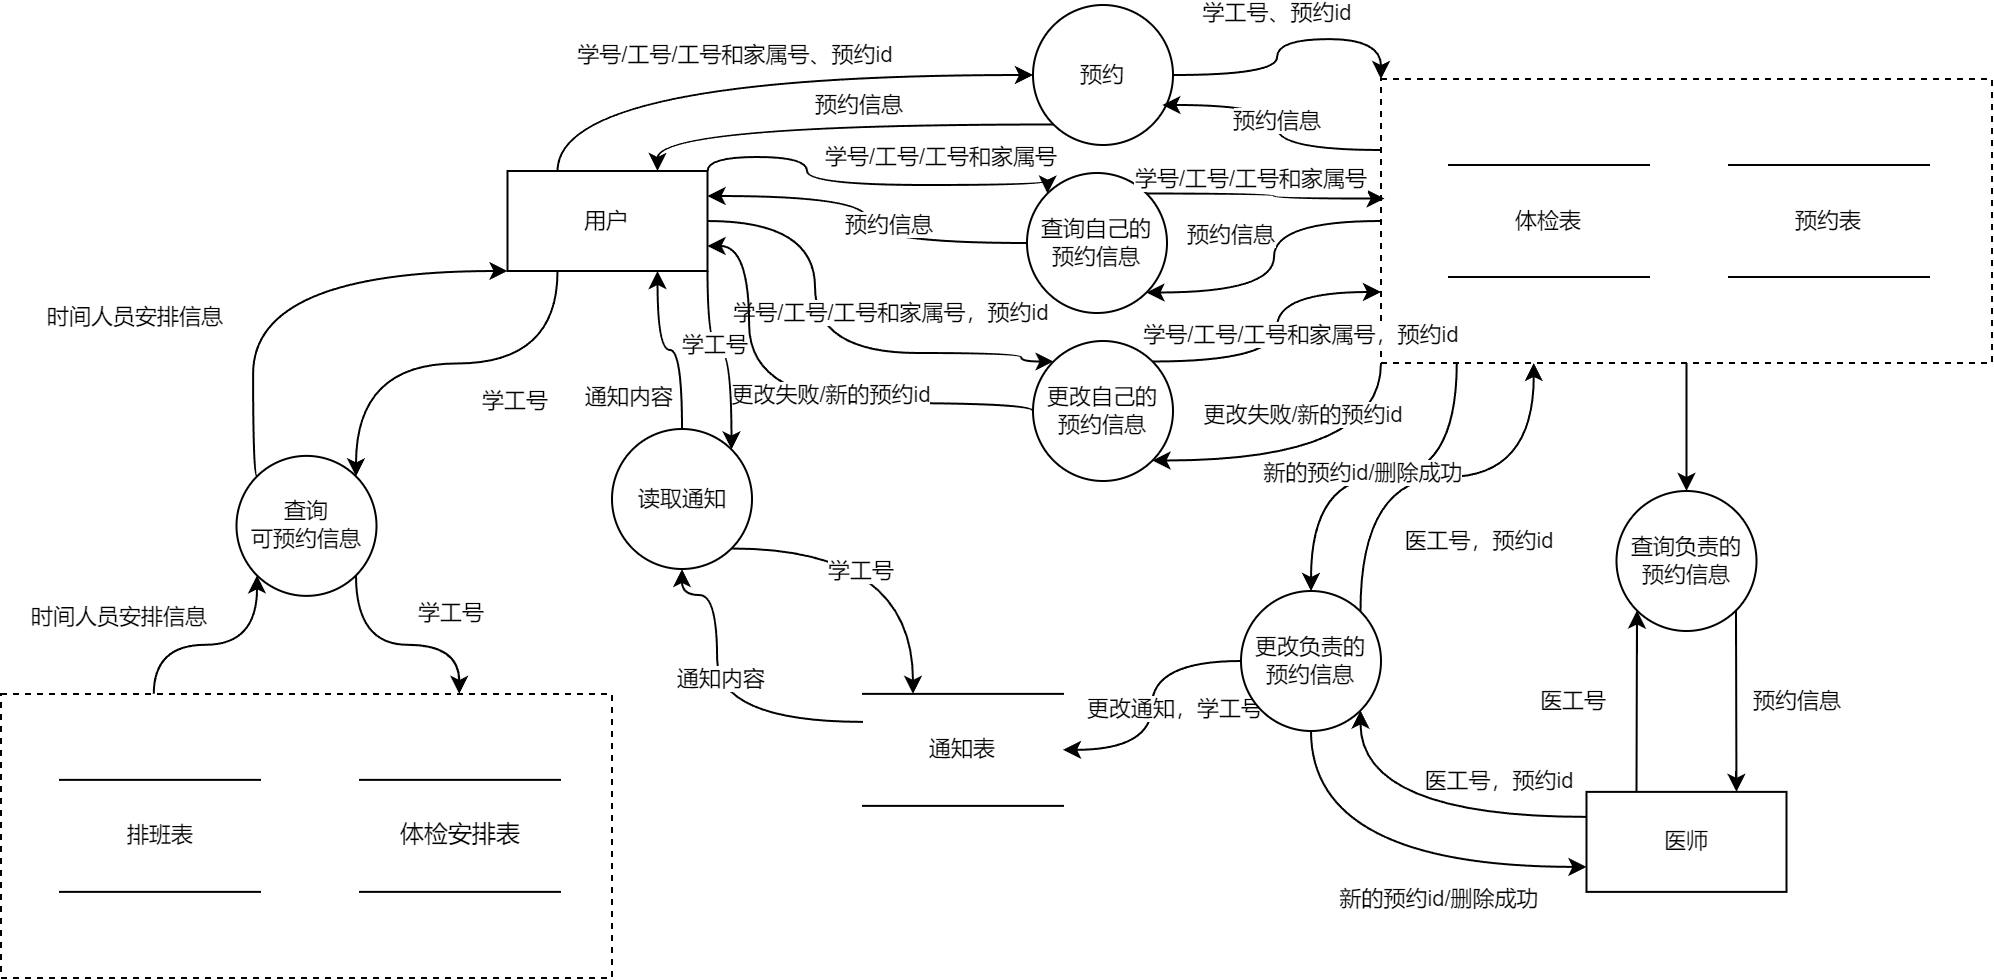
\includegraphics[width=0.8\textwidth]{images/appointment_dataflow.png}
    \caption{预约功能数据流图}
\end{figure}

\paragraph{诊断功能数据流图}

患者在问诊后,医生会进行诊断并诊断结果会保存在数据库中,患者可以查看自己的诊断结果,医生可以查看患者的诊断结果。

\begin{figure}[H]
    \centering
    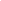
\includegraphics[width=0.8\textwidth]{images/diagnosis_dataflow.png}
    \caption{诊断功能数据流图}
\end{figure}

\paragraph{体检功能数据流图}

患者在体检后,体检结果会保存在数据库中,患者可以查看自己的体检结果,医生可以填写患者的体检结果。

\begin{figure}[H]
    \centering
    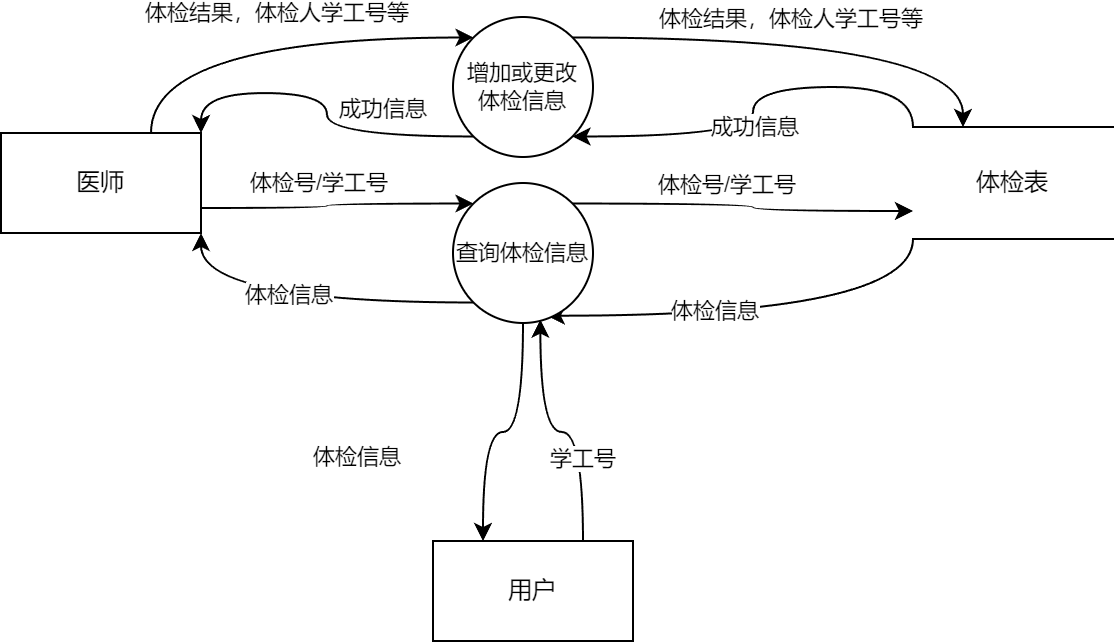
\includegraphics[width=0.8\textwidth]{images/examination_dataflow.png}
    \caption{体检功能数据流图}
\end{figure}

\paragraph{药品管理数据流图}

医生在诊断后,可以开具处方,处方会保存在数据库中,患者可以查看自己的处方,医生可以查看患者的处方。

根据处方,医院会发药,发药信息会保存在数据库中,患者可以查看自己的发药信息。
\begin{figure}[H]
    \centering
    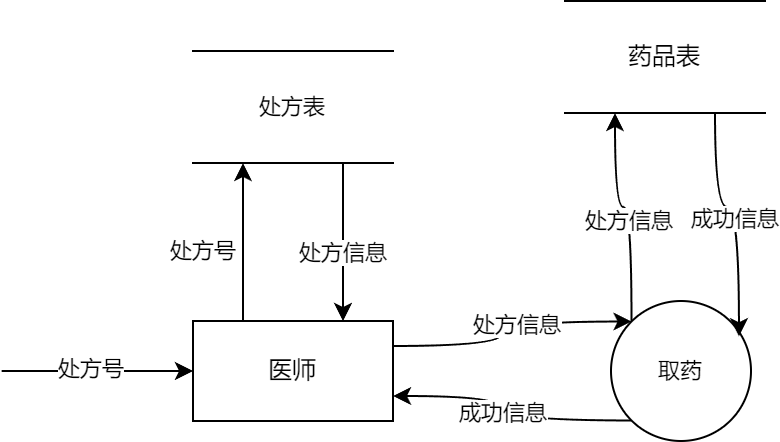
\includegraphics[width=0.7\textwidth]{images/drug_dataflow.png}
    \caption{药品管理数据流图}
\end{figure}

\paragraph{评价功能数据流图}

患者在问诊或者体检后,可以对医生进行评价,评价会保存在数据库中,医生可以查看自己的评价。

\begin{figure}[H]
    \centering
    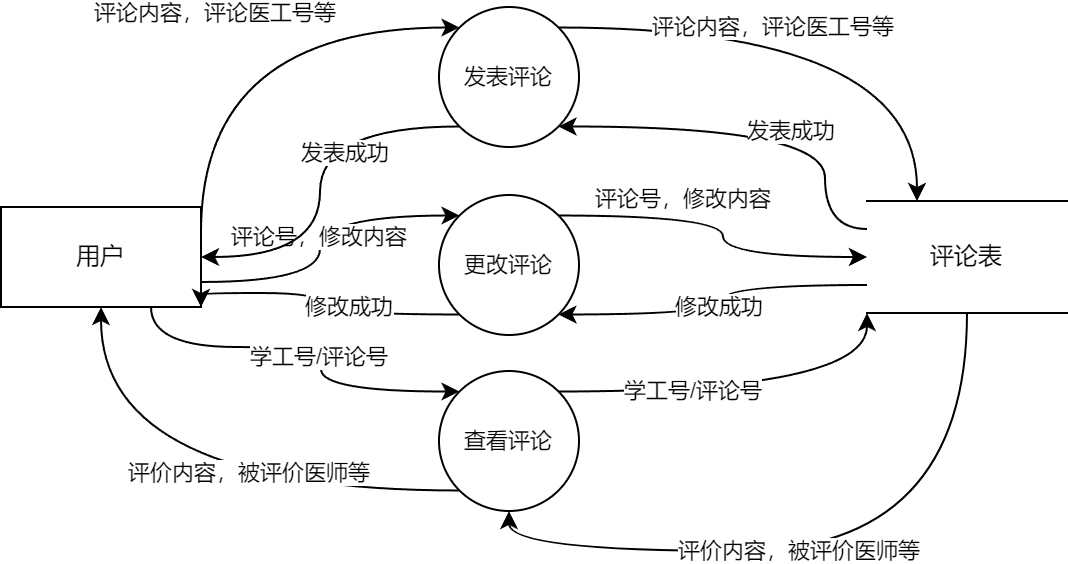
\includegraphics[width=0.8\textwidth]{images/evaluation_dataflow.png}
    \caption{评价功能数据流图}
\end{figure}

\subsection{数据元素表}

\subsubsection{用户管理部分}

\begin{table}[H]
    \centering
    \begin{tabularx}{\textwidth}{|p{2.2cm}|p{3.2cm}|p{4.8cm}|p{5cm}|}
    \toprule
    \textbf{属性名} & \textbf{字段名} & \textbf{含义说明} & \textbf{使用说明} \\ \midrule
    学工号 & id & 用户的学工号 & 作为登录时的账号 \\ \midrule
    密码 & password & 用户的密码 & 注册时设置 \\ \midrule
    姓名 & name & 用户的姓名 & \\ \midrule
    性别 & gender & 用户的性别 &  \\ \midrule
    出生日期 & birth & 用户的出生日期 &  \\ \midrule
    身份证号 & id\_number & 用户的身份证号 &  \\ \midrule
    用户类型 & user\_type & 用户的类型 & s代表学生,t代表老师 \\ \midrule
    手机号 & phone & 用户的手机号 &  \\ \bottomrule
    \end{tabularx}
    \caption{用户数据元素表}
    \label{tab:student_user_elements}
\end{table}

\begin{table}[H]
    \centering
    \begin{tabularx}{\textwidth}{|p{2.2cm}|p{3.2cm}|p{4.8cm}|p{5cm}|}
    \toprule
    \textbf{属性名} & \textbf{字段名} & \textbf{含义说明} & \textbf{使用说明} \\ \midrule
    医工号 & staff\_id & 医生的医工号 & 登录 \\ \midrule
    密码 & password & 医生的密码 & 登录 \\ \midrule
    姓名 & name & 医生的姓名 &  \\ \midrule
    性别 & gender & 医生的性别 &  \\ \midrule
    职称 & title & 医生的职称 &  \\ \midrule
    图片号 & image\_id & 医生的图片号 &  \\ \midrule
    介绍 & introduction & 医生的介绍 &  \\ \bottomrule
    \end{tabularx}
    \caption{医师用户数据元素表}
    \label{tab:doctor_user_elements}
\end{table}

\begin{table}[H]
    \centering
    \begin{tabularx}{\textwidth}{|p{2.2cm}|p{3.3cm}|p{4.7cm}|p{5cm}|}
    \toprule
    \textbf{属性名} & \textbf{字段名} & \textbf{含义说明} & \textbf{使用说明} \\ \midrule
    管理员号 & admin\_id & 管理员的编号 & 登录 \\ \midrule
    姓名 & name & 管理员的姓名 &  \\ \midrule
    密码 & password & 管理员的密码 &  \\ \bottomrule
    \end{tabularx}
    \caption{管理员数据元素表}
    \label{tab:admin_user_elements}
\end{table}

\begin{table}[H]
    \centering
    \begin{tabularx}{\textwidth}{|p{2.2cm}|p{3.3cm}|p{4.7cm}|p{5cm}|}
    \toprule
    \textbf{属性名} & \textbf{字段名} & \textbf{含义说明} & \textbf{使用说明} \\ \midrule
    家属号 & family\_id & 家属的编号 &  \\ \midrule
    学工号 & id & 家属对应的学工号 &  \\ \midrule
    关系 & relationship & 家属与用户的关系 &  \\ \midrule
    姓名 & name & 家属的姓名 &  \\ \midrule
    性别 & gender & 家属的性别 &  \\ \midrule
    出生日期 & birth & 家属的出生日期 &  \\ \midrule
    身份证号 & id\_number & 家属的身份证号 &  \\ \bottomrule
    \end{tabularx}
    \caption{家属数据元素表}
    \label{tab:family_user_elements}
\end{table}

\subsubsection{医疗系统部分}

\begin{table}[H]
    \centering
    \begin{tabularx}{\textwidth}{|p{2.2cm}|p{3.3cm}|p{4.7cm}|p{5cm}|}
    \toprule
    \textbf{属性名} & \textbf{字段名} & \textbf{含义说明} & \textbf{使用说明} \\ \midrule
    科室号 & department\_id & 科室的编号 &  \\ \midrule
    科室名称 & department\_name & 科室的名称 &  \\ \bottomrule
    \end{tabularx}
    \caption{科室数据元素表}
    \label{tab:department_elements}
\end{table}

\begin{table}[H]
    \centering
    \begin{tabularx}{\textwidth}{|p{2.2cm}|p{3.3cm}|p{4.7cm}|p{5cm}|}
    \toprule
    \textbf{属性名} & \textbf{字段名} & \textbf{含义说明} & \textbf{使用说明} \\ \midrule
    排班号 & schedule\_id & 排班的编号 &  \\ \midrule
    医工号 & staff\_id & 医生的医工号 &  \\ \midrule
    科室号 & department\_id & 科室的编号 &  \\ \midrule
    排班时间 & schedule\_time & 排班的时间 &  \\ \bottomrule
    \end{tabularx}
    \caption{排班数据元素表}
    \label{tab:schedule_elements}
\end{table}

\begin{table}[H]
    \centering
    \begin{tabularx}{\textwidth}{|p{2.2cm}|p{3.3cm}|p{4.7cm}|p{5cm}|}
    \toprule
    \textbf{属性名} & \textbf{字段名} & \textbf{含义说明} & \textbf{使用说明} \\ \midrule
    药房号 & pharmacy\_id & 药房的编号 &  \\ \midrule
    药房名称 & pharmacy\_name & 药房的名称 &  \\ \bottomrule
    \end{tabularx}
    \caption{药房数据元素表}
    \label{tab:pharmacy_elements}
\end{table}

\begin{table}[H]
    \centering
    \begin{tabularx}{\textwidth}{|p{2.2cm}|p{3.3cm}|p{4.7cm}|p{5cm}|}
    \toprule
    \textbf{属性名} & \textbf{字段名} & \textbf{含义说明} & \textbf{使用说明} \\ \midrule
    药品号 & drug\_id & 药品的编号 &  \\ \midrule
    药品名称 & drug\_name & 药品的名称 &  \\ \midrule
    药品价格 & price & 药品的价格 &  \\ \bottomrule
    \end{tabularx}
    \caption{药品数据元素表}
    \label{tab:drug_elements}
\end{table}

\begin{table}[H]
    \centering
    \begin{tabularx}{\textwidth}{|p{2.2cm}|p{3.3cm}|p{4.7cm}|p{5cm}|}
    \toprule
    \textbf{属性名} & \textbf{字段名} & \textbf{含义说明} & \textbf{使用说明} \\ \midrule
    药品号 & drug\_id & 药品的编号 &  \\ \midrule
    药品数量 & drug\_amount & 药品的数量 &  \\ \midrule
    药房号 & pharmacy\_id & 药房的编号 &  \\ \bottomrule
    \end{tabularx}
    \caption{药品库存数据元素表}
    \label{tab:drug_storage_elements}
\end{table}

\subsubsection{预约管理部分}

\begin{table}[H]
    \centering
    \begin{tabularx}{\textwidth}{|p{2.2cm}|p{3.3cm}|p{4.7cm}|p{5cm}|}
    \toprule
    \textbf{属性名} & \textbf{字段名} & \textbf{含义说明} & \textbf{使用说明} \\ \midrule
    体检号 & examination\_id & 体检的编号 &  \\ \midrule
    体检项目 & examination & 体检的项目 &  \\ \midrule
    体检日期 & examination\_date & 体检的日期 &  \\ \midrule
    负责医工号 & staff\_id & 负责体检的医生的医工号 &  \\ \bottomrule
    \end{tabularx}
    \caption{体检安排数据元素表}
    \label{tab:examination_arrangement_elements}
\end{table}

\begin{table}[H]
    \centering
    \begin{tabularx}{\textwidth}{|p{2.2cm}|p{3.3cm}|p{4.7cm}|p{5cm}|}
    \toprule
    \textbf{属性名} & \textbf{字段名} & \textbf{含义说明} & \textbf{使用说明} \\ \midrule
    体检预约号 & exam\_appointment\_id & 体检预约的编号 &  \\ \midrule
    体检号 & examination\_id & 体检的编号 &  \\ \midrule
    体检结果 & examination\_result & 体检的结果 &  \\ \midrule
    学工号 & id & 学工号 &  \\ \bottomrule
    \end{tabularx}
    \caption{体检信息数据元素表}
    \label{tab:examination_appointment_elements}
\end{table}

\begin{table}[H]
    \centering
    \begin{tabularx}{\textwidth}{|p{2.2cm}|p{3.3cm}|p{4.7cm}|p{5cm}|}
    \toprule
    \textbf{属性名} & \textbf{字段名} & \textbf{含义说明} & \textbf{使用说明} \\ \midrule
    预约号 & appointment\_id & 预约的编号 &  \\ \midrule
    患者与预约人关系 & relationship & 患者与预约人的关系 &  \\ \midrule
    排班号 & schedule\_id & 排班的编号 &  \\ \midrule
    学工号 & id & 学工号 &  \\ \bottomrule
    \end{tabularx}
    \caption{预约数据元素表}
    \label{tab:appointment_elements}
\end{table}

\begin{table}[H]
    \centering
    \begin{tabularx}{\textwidth}{|p{2.2cm}|p{3.3cm}|p{4.7cm}|p{5cm}|}
    \toprule
    \textbf{属性名} & \textbf{字段名} & \textbf{含义说明} & \textbf{使用说明} \\ \midrule
    诊断号 & diagnosis\_id & 诊断的编号 &  \\ \midrule
    检查项目 & examination & 诊断的项目 &  \\ \midrule
    检查结果 & examination\_result & 诊断的结果 &  \\ \midrule
    参考范围 & reference & 诊断的参考范围 &  \\ \midrule
    临床诊断 & clinical\_diagnosis & 诊断的临床诊断 &  \\ \midrule
    处方号 & prescription\_id & 处方的编号 &  \\ \midrule
    诊断时间 & diagnosis\_time & 诊断的时间 &  \\ \midrule
    患者身份证号 & id\_number & 患者的身份证号 &  \\ \midrule
    预约号 & appointment\_id & 预约的编号 &  \\ \midrule
    医工号 & staff\_id & 医生的医工号 &  \\ \bottomrule
    \end{tabularx}
    \caption{诊断数据元素表}
    \label{tab:diagnosis_elements}
\end{table}

\subsubsection{药品管理部分}

\begin{table}[H]
    \centering
    \begin{tabularx}{\textwidth}{|p{2.2cm}|p{3.3cm}|p{4.7cm}|p{5cm}|}
    \toprule
    \textbf{属性名} & \textbf{字段名} & \textbf{含义说明} & \textbf{使用说明} \\ \midrule
    处方号 & prescription\_id & 处方的编号 &  \\ \midrule
    诊断号 & diagnosis\_id & 诊断的编号 &  \\ \midrule
    药品号 & drug\_id & 药品的编号 &  \\ \midrule
    药品数量 & drug\_amount & 药品的数量 &  \\ \midrule
    用法用量 & usage & 药品的用法用量 &  \\ \midrule
    注意事项 & precautions & 药品的注意事项 &  \\ \bottomrule
    \end{tabularx}
    \caption{处方数据元素表}
    \label{tab:prescription_elements}
\end{table}

\subsubsection{其他数据元素}

\begin{table}[H]
    \centering
    \begin{tabularx}{\textwidth}{|p{2.2cm}|p{3.3cm}|p{4.7cm}|p{5cm}|}
    \toprule
    \textbf{属性名} & \textbf{字段名} & \textbf{含义说明} & \textbf{使用说明} \\ \midrule
    通知号 & notification\_id & 通知的编号 &  \\ \midrule
    通知内容 & notification & 通知的内容 &  \\ \midrule
    通知时间 & notification\_time & 通知的时间 &  \\ \midrule
    接收人学工号 & staff\_id & 接收人的学工号 &  \\ \bottomrule
    \end{tabularx}
    \caption{通知数据元素表}
    \label{tab:notification_elements}
\end{table}

\begin{table}[H]
    \centering
    \begin{tabularx}{\textwidth}{|p{2.2cm}|p{3.3cm}|p{4.7cm}|p{5cm}|}
    \toprule
    \textbf{属性名} & \textbf{字段名} & \textbf{含义说明} & \textbf{使用说明} \\ \midrule
    评价号 & evaluation\_id & 评价的编号 &  \\ \midrule
    评价内容 & evaluation & 评价的内容 &  \\ \midrule
    评价时间 & evaluation\_time & 评价的时间 &  \\ \midrule
    评价人学工号 & id & 评价人的学工号 &  \\ \midrule
    被评价人医工号 & staff\_id & 被评价人的医工号 &  \\ \bottomrule
    \end{tabularx}
    \caption{评价数据元素表}
    \label{tab:evaluation_elements}
\end{table}

\begin{table}[H]
    \centering
    \begin{tabularx}{\textwidth}{|p{2.2cm}|p{3.3cm}|p{4.7cm}|p{5cm}|}
    \toprule
    \textbf{属性名} & \textbf{字段名} & \textbf{含义说明} & \textbf{使用说明} \\ \midrule
    图片号 & image\_id & 图片的编号 &  \\ \midrule
    存储路径 & image\_path & 图片的存储路径 &  \\ \midrule
    评价号 & evaluation\_id & 评价的编号 &  \\ \midrule
    通知号 & notification\_id & 通知的编号 &  \\ \midrule
    药品号 & drug\_id & 药品的编号 &  \\ \bottomrule
    \end{tabularx}
    \caption{图片数据元素表}
    \label{tab:image_elements}
\end{table}

\section{数据库概念模式设计}

\subsection{系统分E-R 图}

一个用户(用户类型为教职工)可以有多个家属,一个家属只能对应一个用户。

\begin{figure}[H]
    \centering
    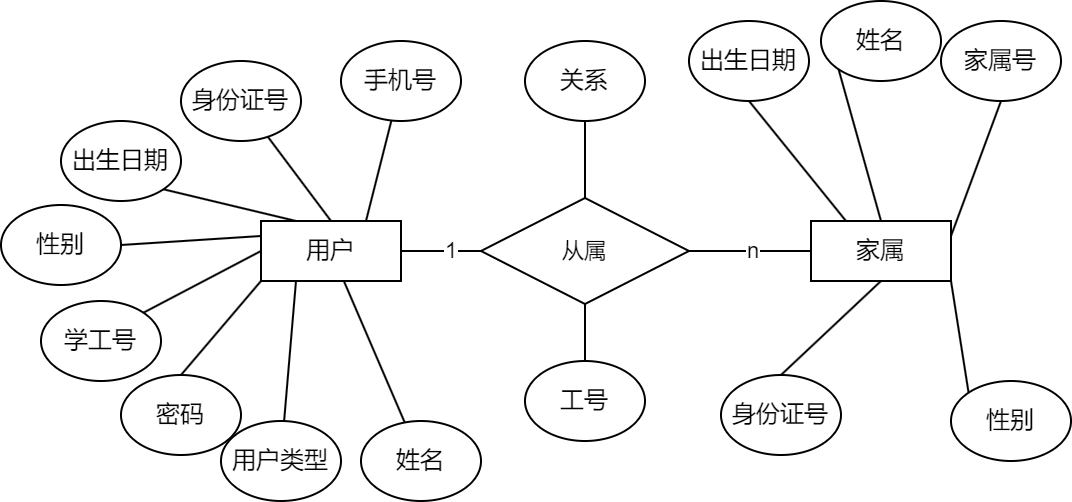
\includegraphics[width=0.8\textwidth]{images/dividedER1.png}
    \caption{系统分 E-R 图}
\end{figure}

一个医院管理员可以安排多个医生的排班,一个医生可以被安排多个排班。
一个科室可以有多个医生,一个医生只能属于一个科室。
一个科室可以有多个排班信息,一个排班信息只能属于一个科室。

\begin{figure}[H]
    \centering
    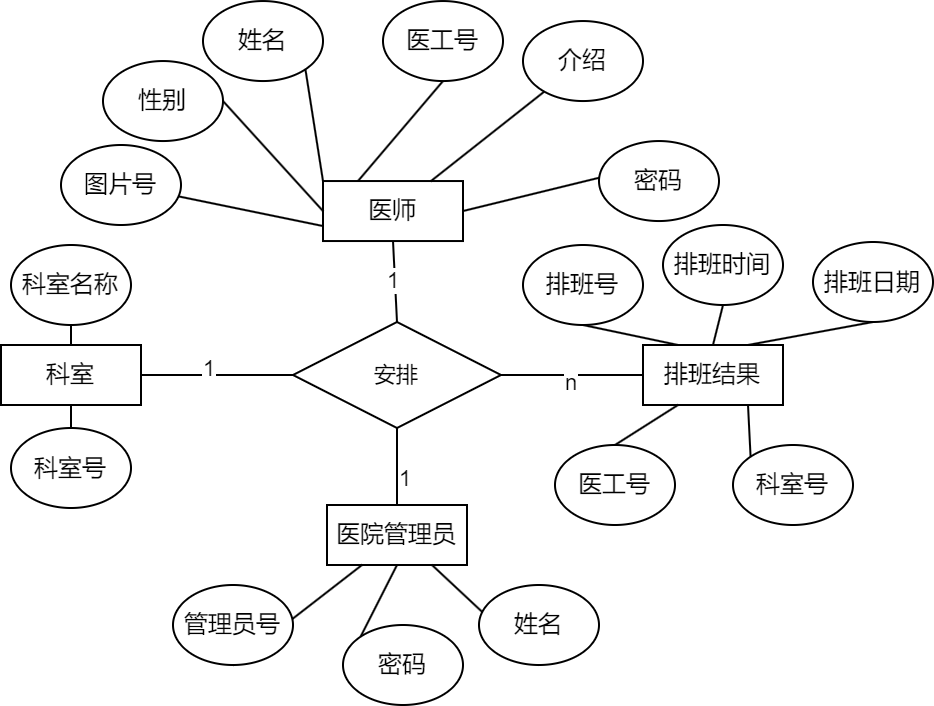
\includegraphics[width=0.8\textwidth]{images/dividedER2.png}
    \caption{系统分 E-R 图}
\end{figure}

一个诊断可以有多个处方,一个处方只能对应一个诊断。

\begin{figure}[H]
    \centering
    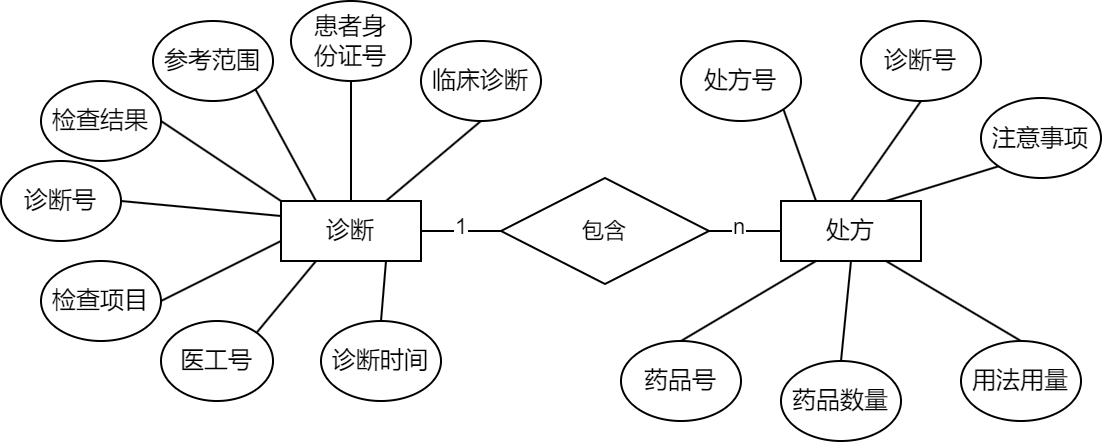
\includegraphics[width=0.8\textwidth]{images/dividedER3.png}
    \caption{系统分 E-R 图}
\end{figure}

一个药品只会在一个药房,一个药房可以有多个药品。
一次体检安排可以有多个体检结果,一个体检结果只能对应一个体检安排。

\begin{figure}[H]
    \centering
    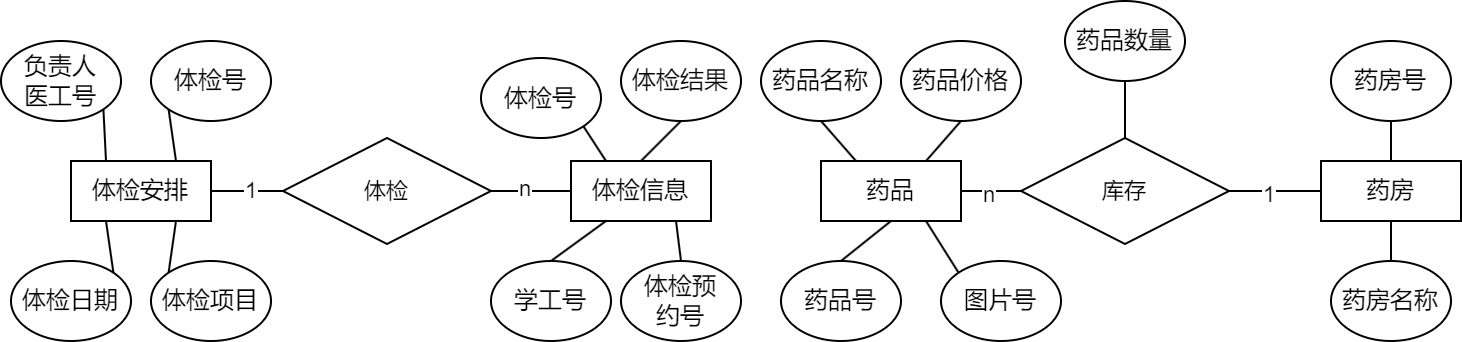
\includegraphics[width=0.8\textwidth]{images/dividedER4.png}
    \caption{系统分 E-R 图}
\end{figure}

一个医院管理员可以发送多个通知,一个用户可以接收多个通知。
一个用户可以发送多个评价,一个评价只属于一个用户,一个医生可以接收多个评价。
一个用户可以发起多个预约,一个预约只属于一个排班,一个排班可以有多个预约。

\begin{figure}[H]
    \centering
    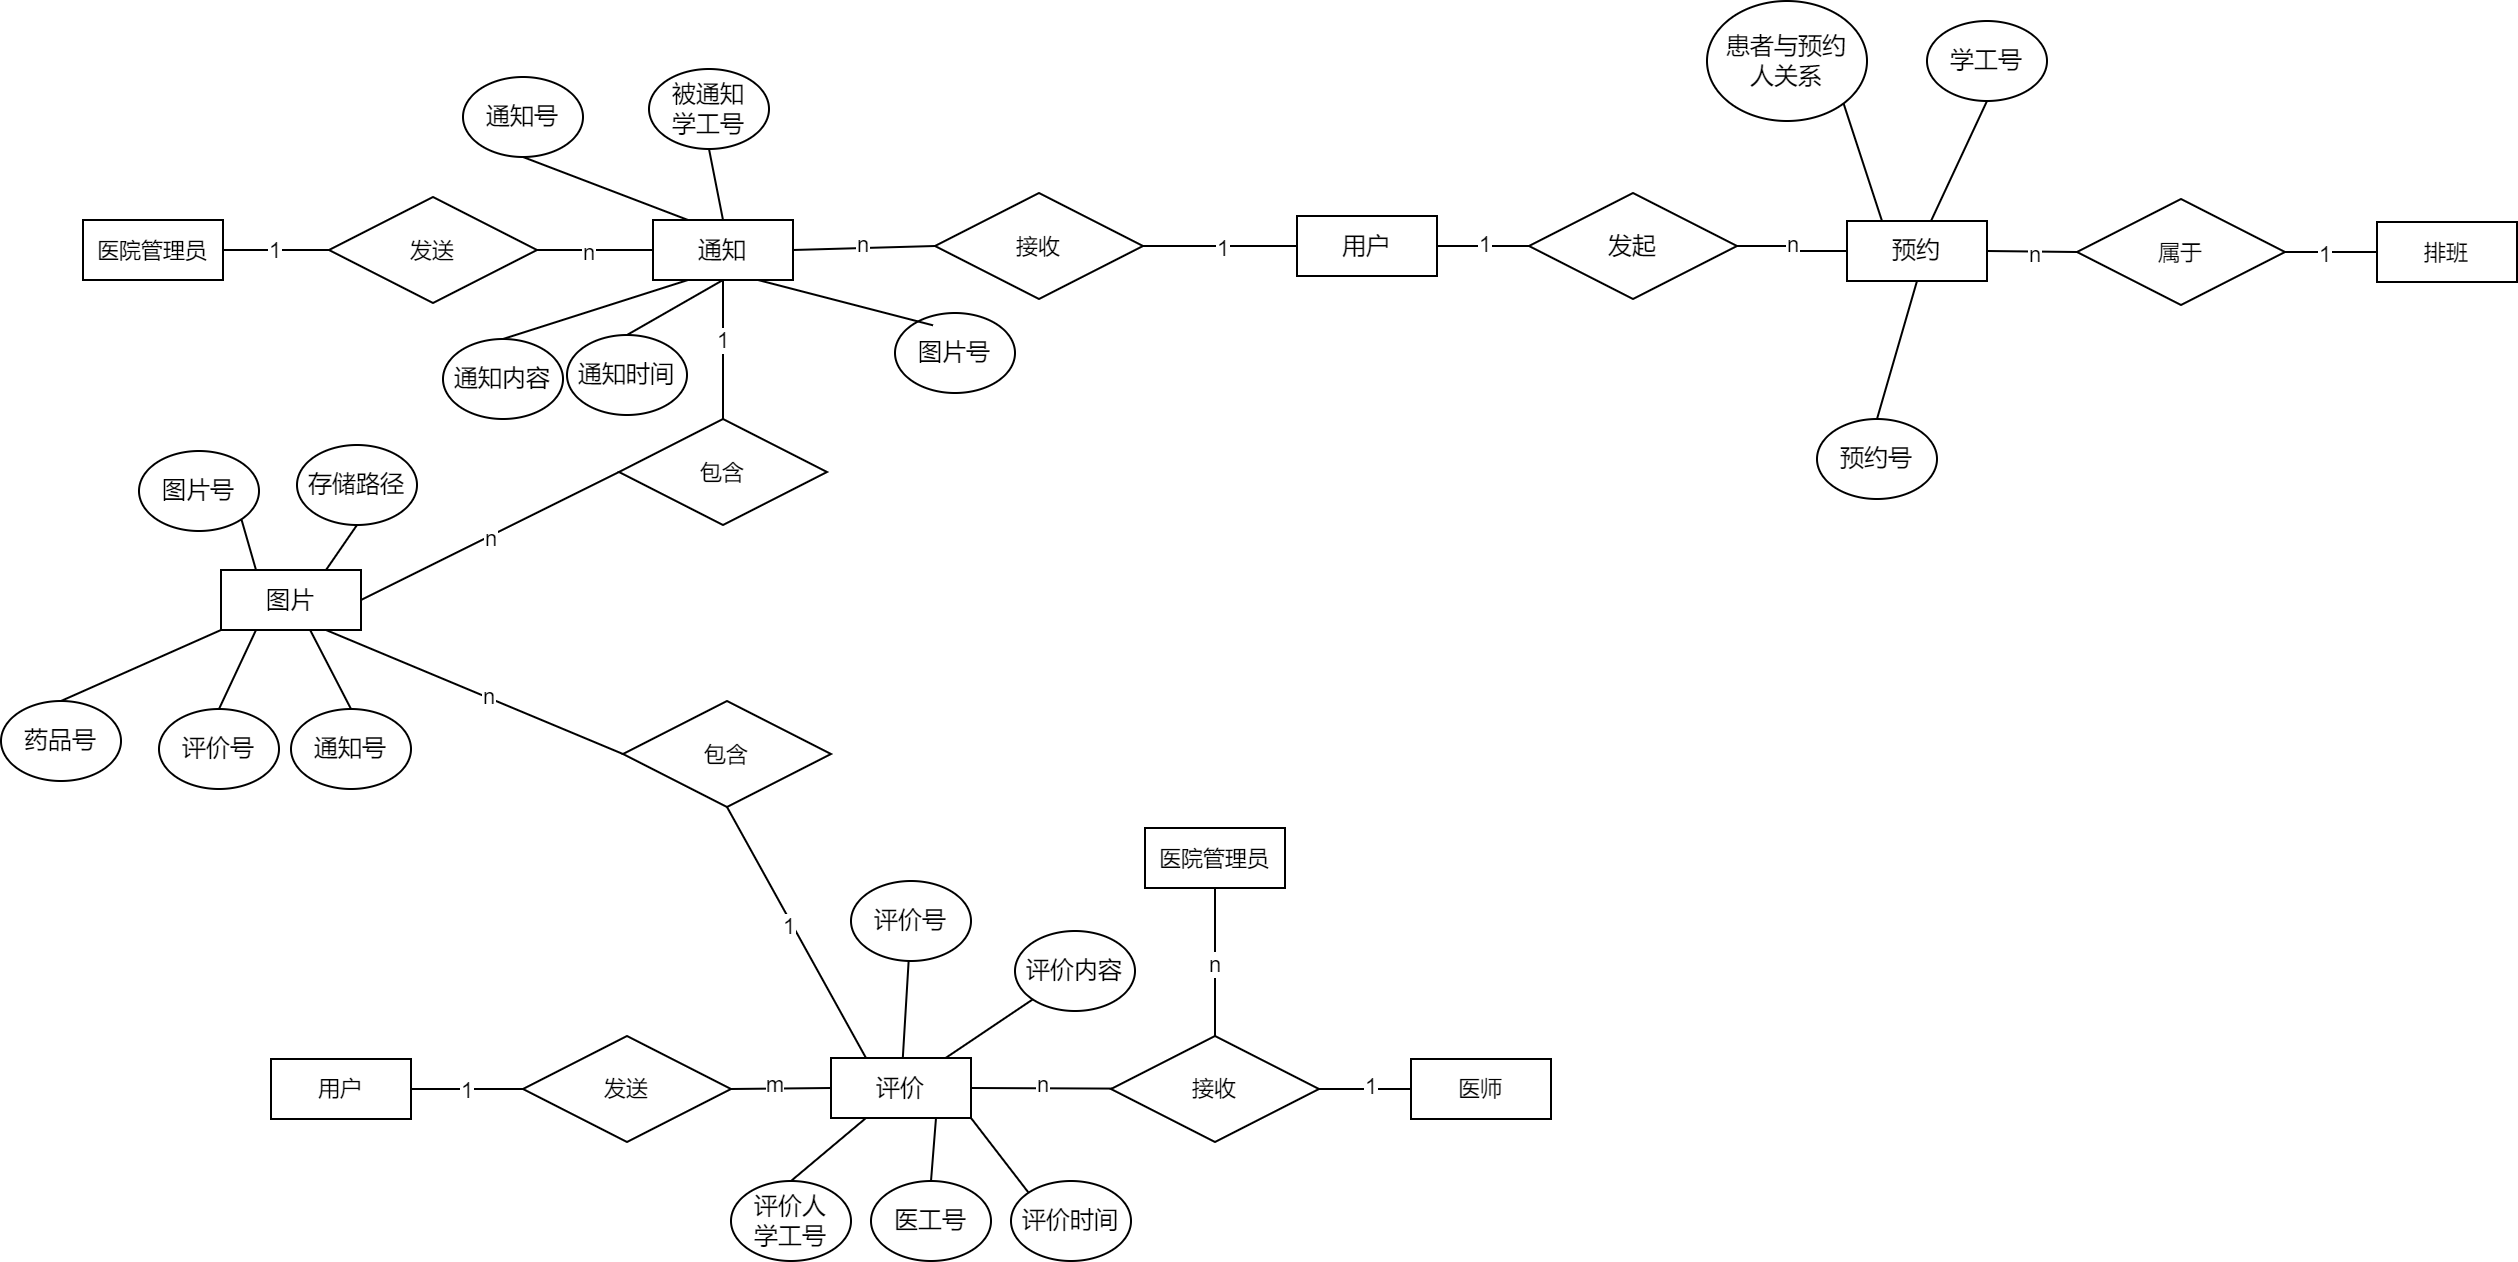
\includegraphics[width=0.8\textwidth]{images/dividedER5.png}
    \caption{系统分 E-R 图}
\end{figure}

\subsection{系统初步E-R 图}

可以得到系统的初步 E-R 图如下(已经略去属性,详见分 E-R 图):

\begin{figure}[H]
    \centering
    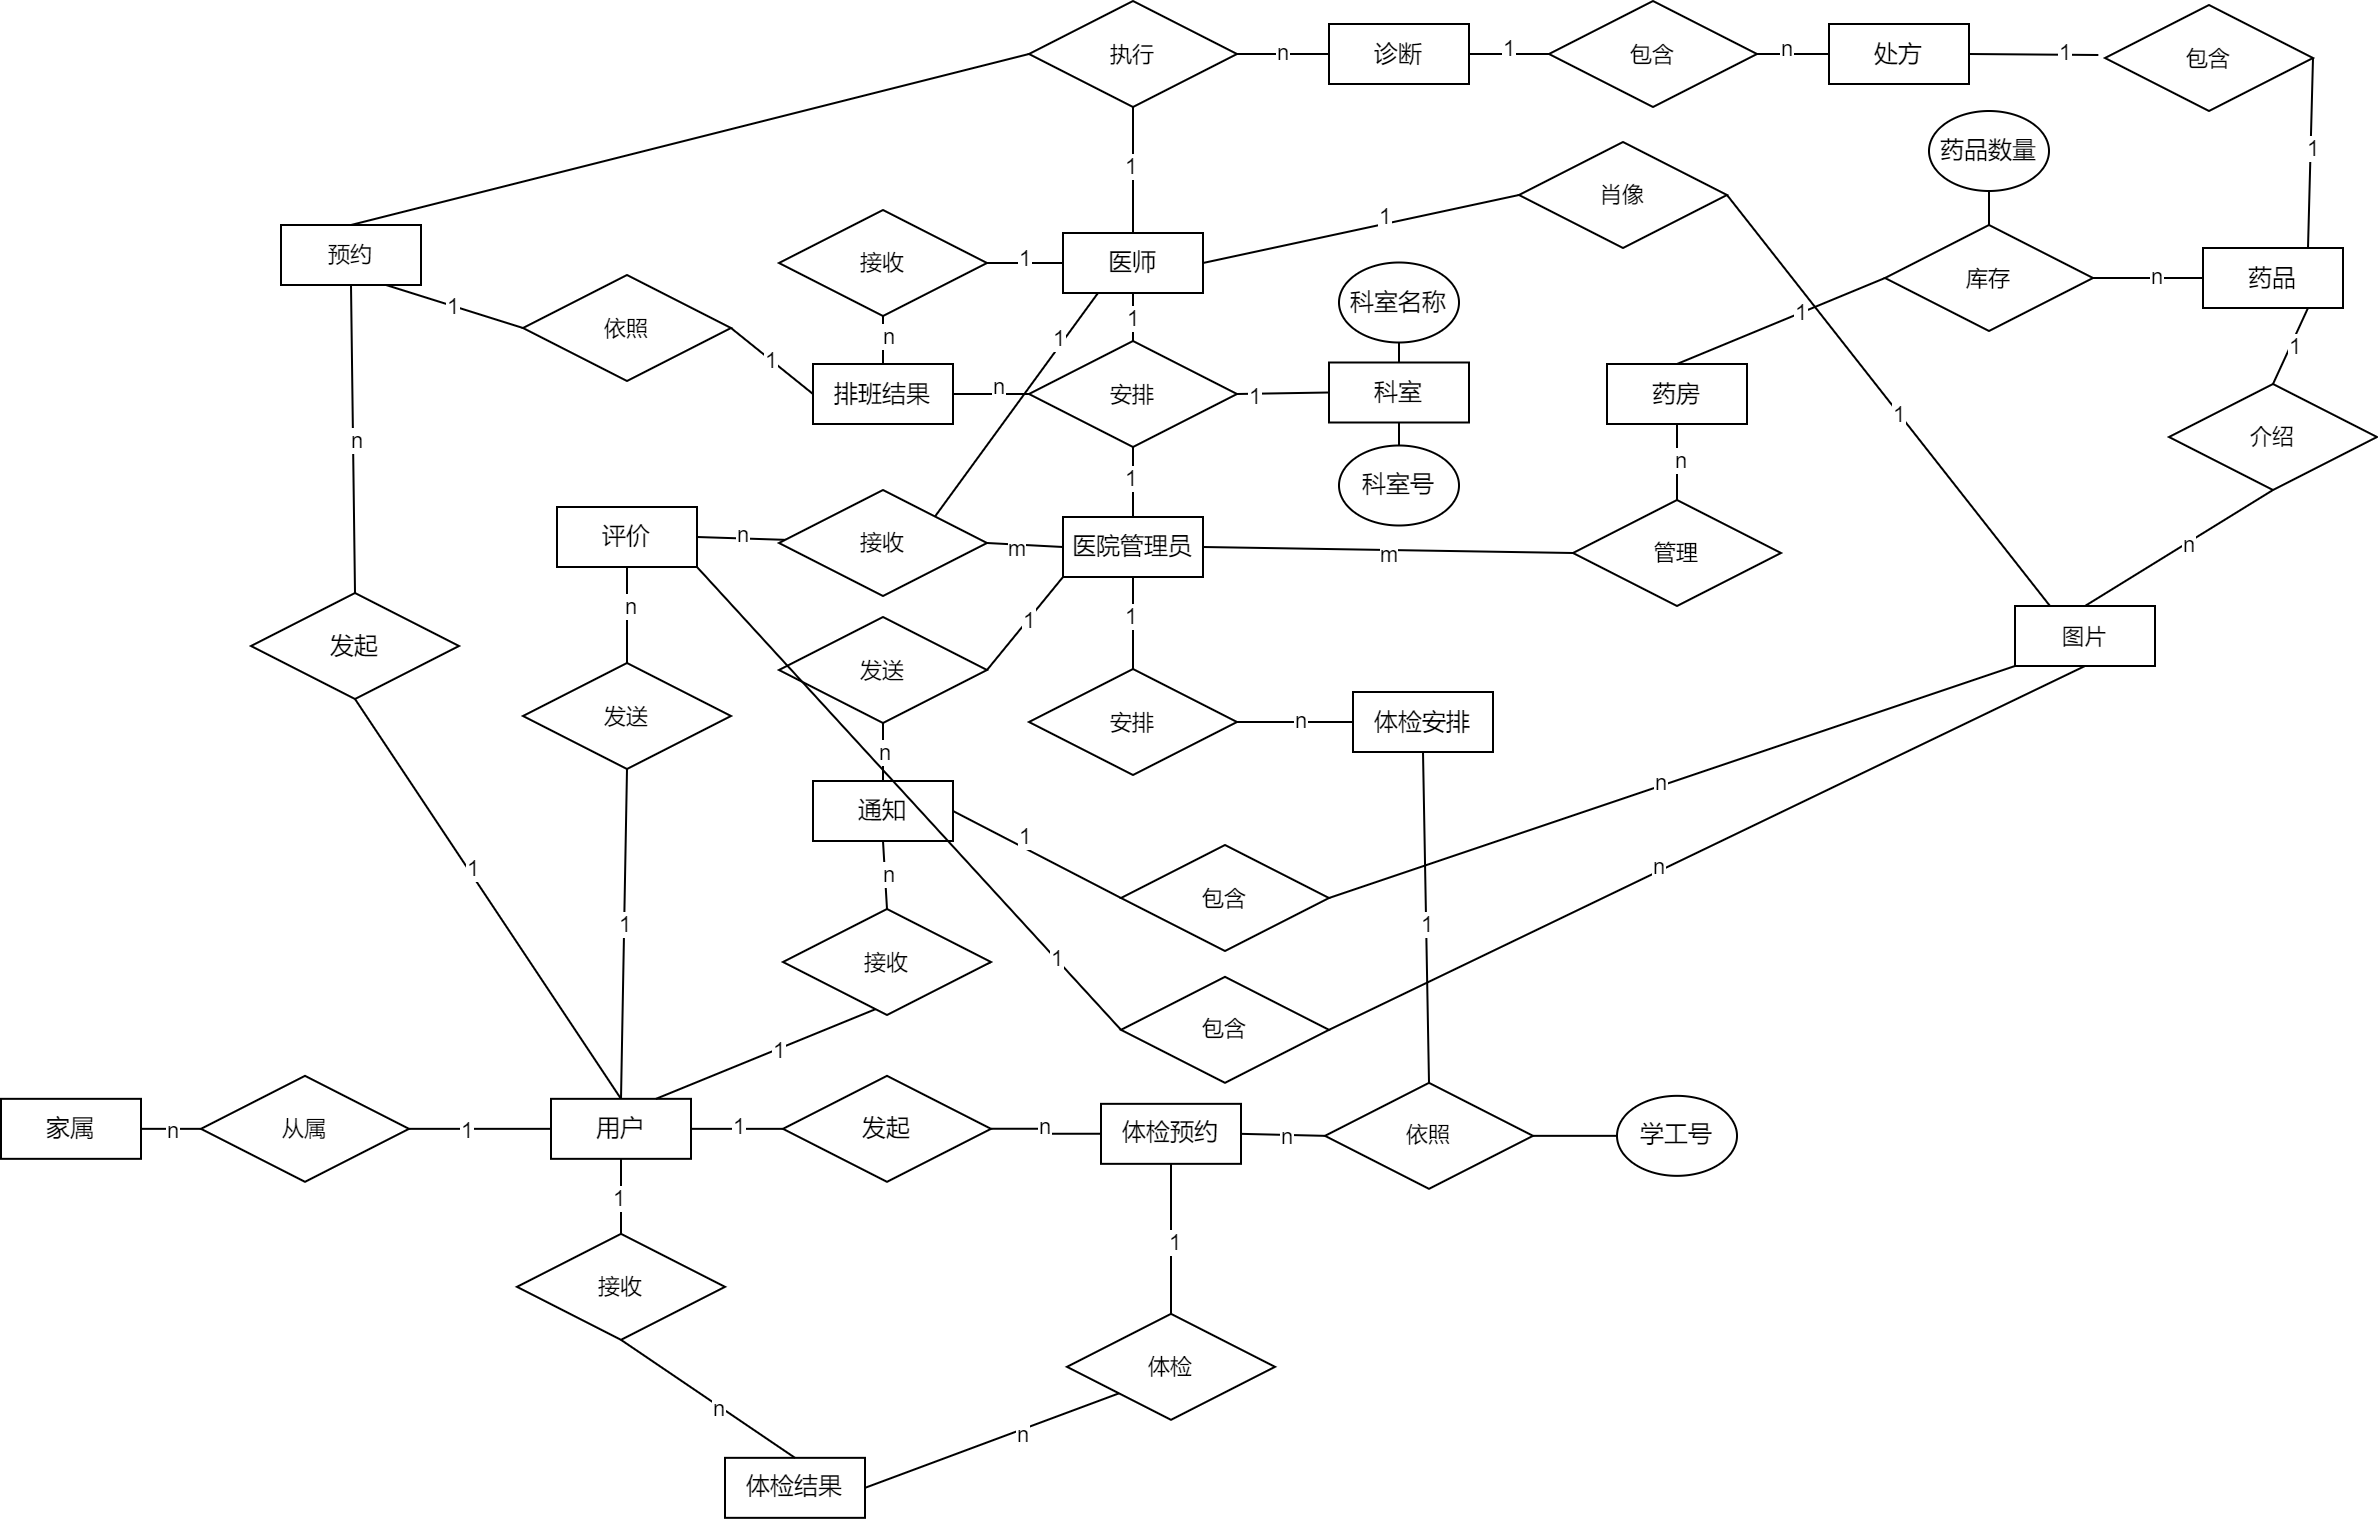
\includegraphics[width=0.8\textwidth]{images/initER.png}
    \caption{系统初步 E-R 图}
\end{figure}

\subsection{系统基本 E-R 图}

由于医师,医生管理员和科室是1:1:1的关系,我们可以将实体科室下降为医生管理员安排医师排班这一关系的属性,而科室的属性直接降为这一关系的属性。

可以得到系统的基本 E-R 图如下(已经略去属性,详见分 E-R 图):

\begin{figure}[H]
    \centering
    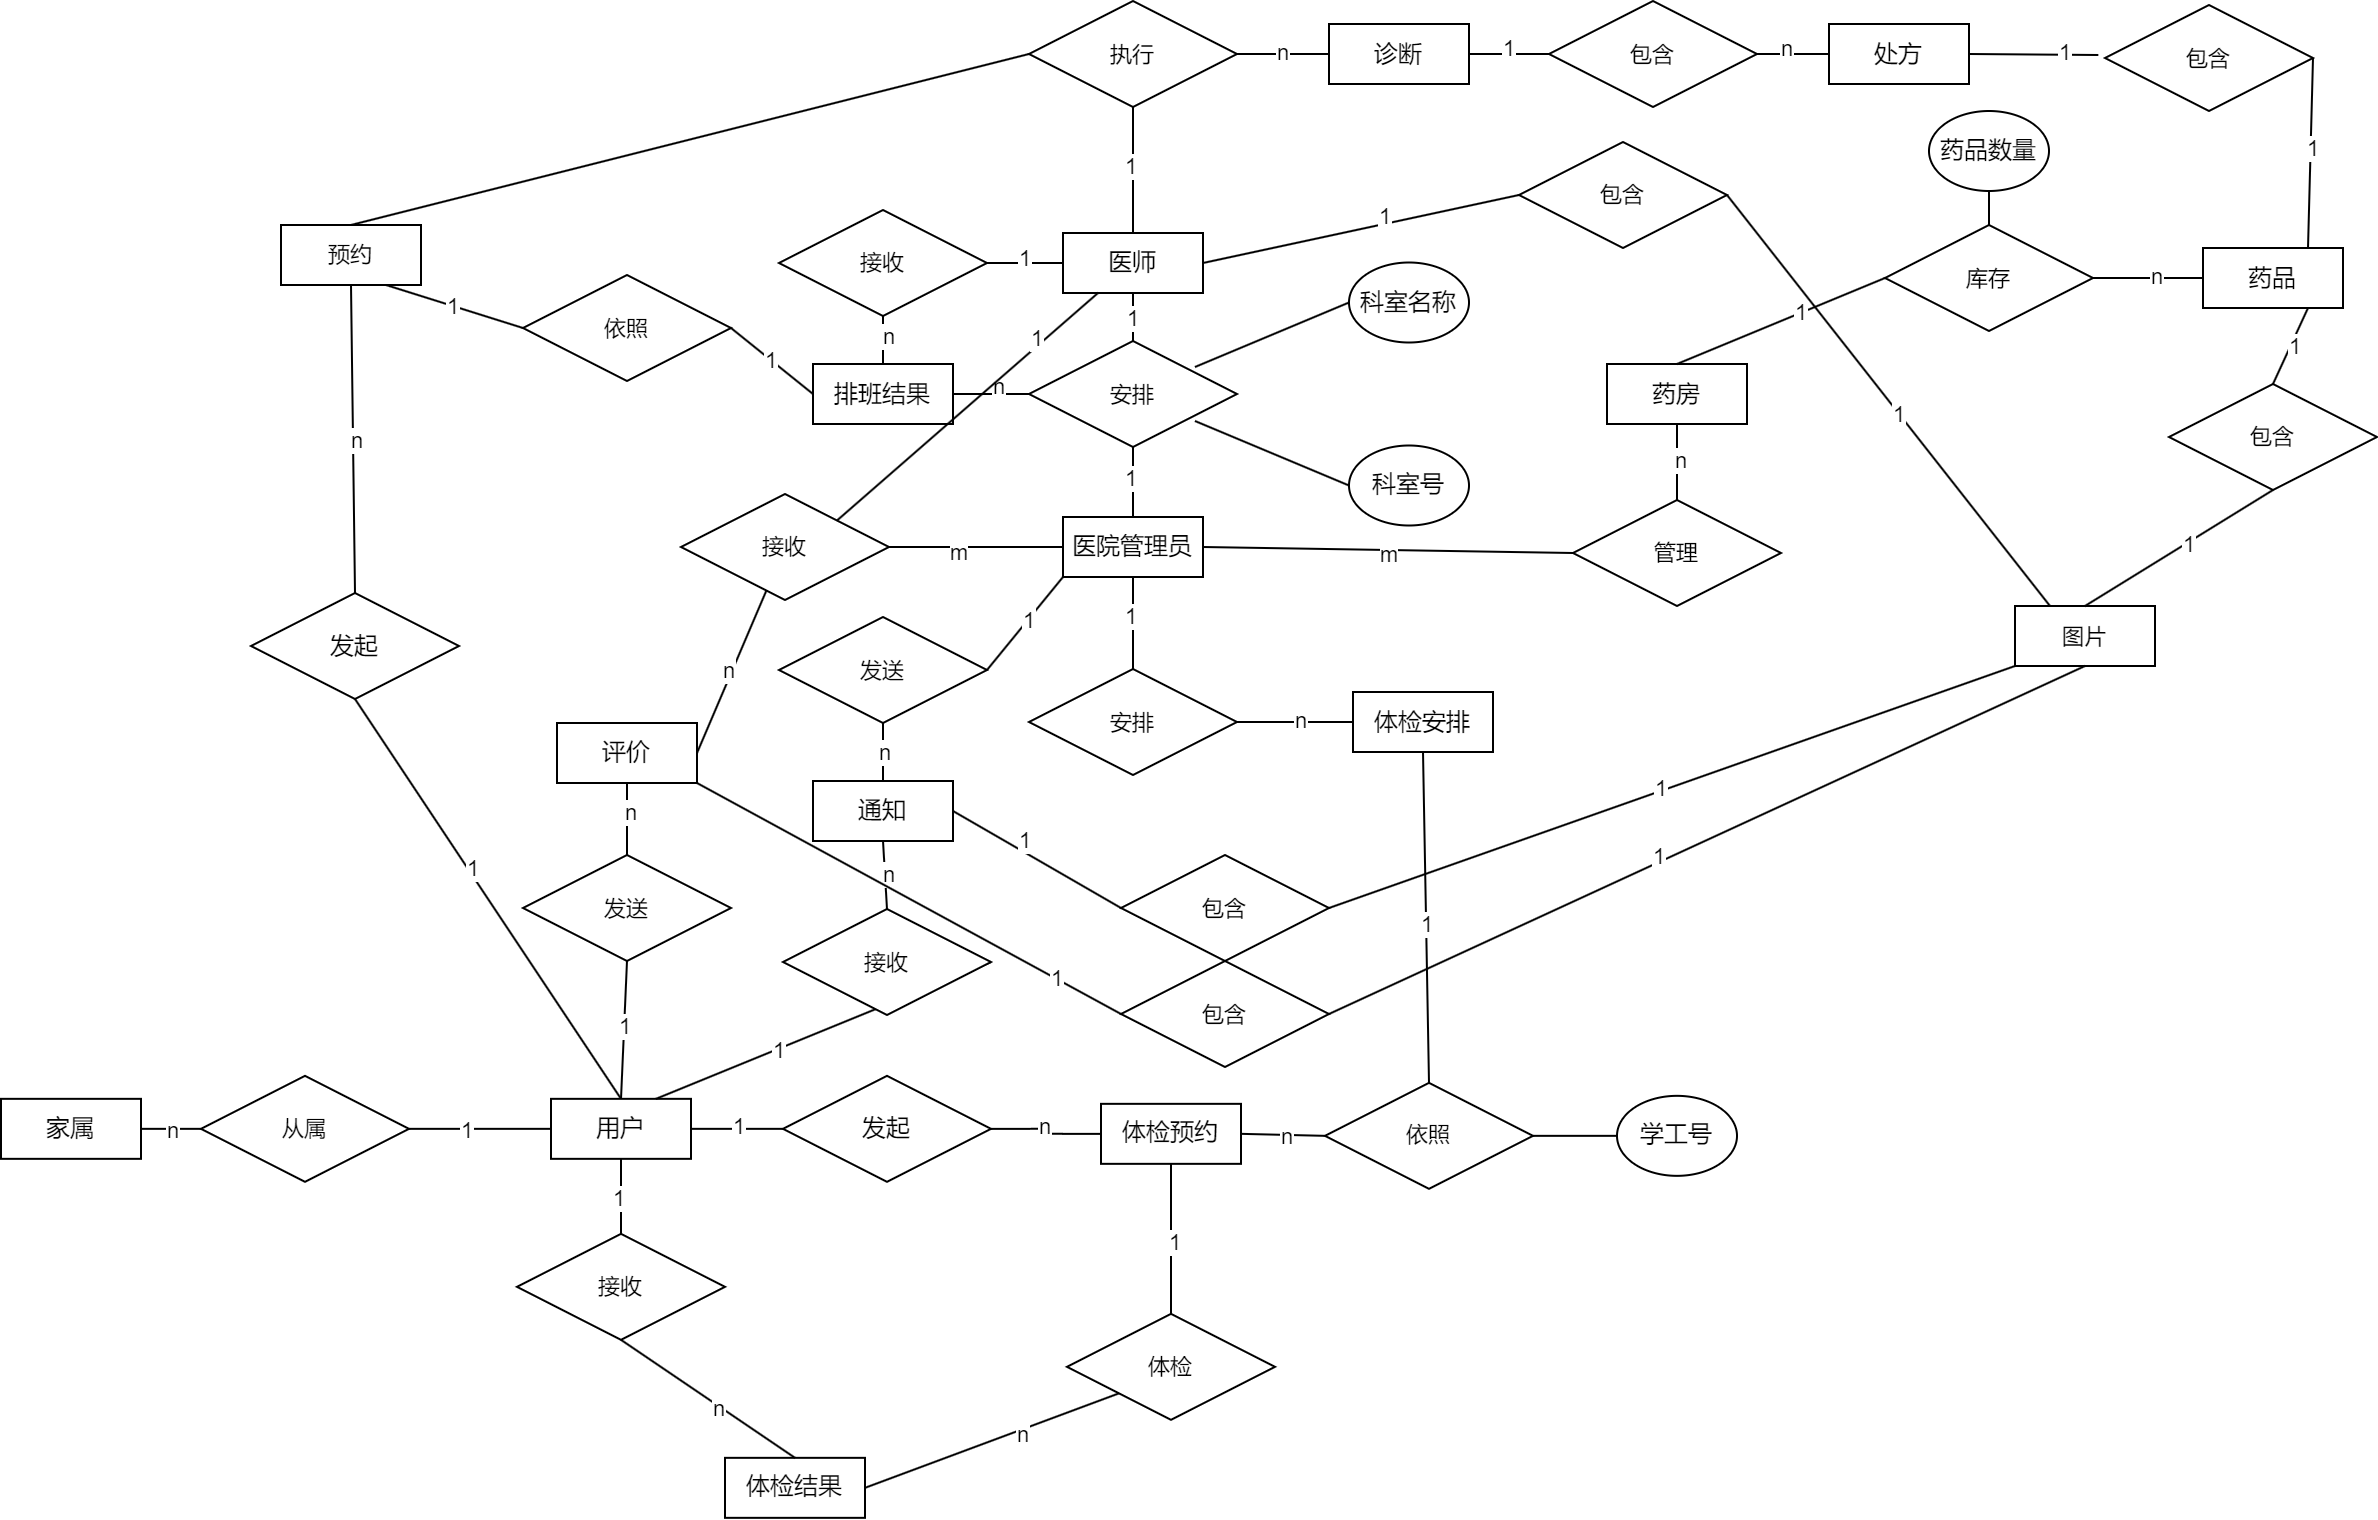
\includegraphics[width=0.8\textwidth]{images/basicER.png}
    \caption{系统基本 E-R 图}
\end{figure}

\section{数据库逻辑模式设计与优化}
\subsection{数据库关系模式定义}
关系模式可以形式化表⽰为 $R(U, D, DOM, F)$ 。$U$ 为组成该关系的属性名,$D$ 为 $U$ 中属性所来⾃的域,
$DOM$ 指的是属性与域的映射,$F$ 指的是属性间的依赖关系集合。以下约定 $N$ 表示正整数,$S$ 表示任意字符组成的字符串, $T$ 表示时间, $DT$代表日期。码以下划线标识。

下面是由 ER 图得到的关系模式。

\subsubsection{实体}

\paragraph{用户}

用户(\{\underline{学工号}, 密码, 姓名, 性别, 出生日期, 身份证号, 用户类型, 手机号\}, $D_{user}$, $DOM_{user}$, $F_{user}$)

D\_user = \{S,DT\}

DOM\_user = \{DOM\_user(学工号) = DOM\_user(密码) = DOM\_user(姓名) = DOM\_user(性别) = DOM\_user(身份证号) = DOM\_user(用户类型) = DOM\_user(手机号) = S , DOM\_user(出生日期) = DT\}

F\_user = \{学工号 $\rightarrow$ 密码, 姓名, 性别, 出生日期, 身份证号, 用户类型, 手机号\}

\paragraph{家属}

家属(\{\underline{家属号}, 姓名, 性别, 出生日期, 身份证号\}, $D_{family}$, $DOM_{family}$, $F_{family}$)

D\_family = \{S,DT\}

DOM\_family = \{DOM\_family(家属号) = DOM\_family(姓名) = DOM\_family(性别) = DOM\_family(身份证号) = S, DOM\_family(出生日期) = DT\}

F\_family = \{家属号 $\rightarrow$ 姓名, 性别, 出生日期, 身份证号\}

\paragraph{医师}

医师(\{\underline{医工号}, 密码, 姓名, 性别, 职称, 图片号, 介绍\}, $D_{doctor}$, $DOM_{doctor}$, $F_{doctor}$)

D\_doctor = \{S\}

DOM\_doctor = \{DOM\_doctor(医工号) = DOM\_doctor(密码) = DOM\_doctor(姓名) = \newline DOM\_doctor(性别) = DOM\_doctor(职称) = DOM\_doctor(图片号) = DOM\_doctor(介绍) = S\}

F\_doctor = \{医工号 $\rightarrow$ 密码, 姓名, 性别, 职称, 图片号, 介绍\}

\paragraph{医院管理员}

医院管理员(\{\underline{管理员号}, 密码, 姓名\}, $D_{admin}$, $DOM_{admin}$, $F_{admin}$)

D\_admin = \{S\}

DOM\_admin = \{DOM\_admin(管理员号) = DOM\_admin(密码) = DOM\_admin(姓名) = S\}

F\_admin = \{管理员号 $\rightarrow$ 密码, 姓名\}

\paragraph{科室}

科室(\{\underline{科室号}, 科室名称\}, $D_{department}$, $DOM_{department}$, $F_{department}$)

D\_department = \{S\}

DOM\_department = \{DOM\_department(科室号) = DOM\_department(科室名称) = S\}

F\_department = \{科室号 $\rightarrow$ 科室名称\}

\paragraph{药房}

药房(\{\underline{药房号}, 药房名称\}, $D_{pharmacy}$, $DOM_{pharmacy}$, $F_{pharmacy}$)

D\_pharmacy = \{S\}

DOM\_pharmacy = \{DOM\_pharmacy(药房号) = DOM\_pharmacy(药房名称) = S\}

F\_pharmacy = \{药房号 $\rightarrow$ 药房名称\}

\paragraph{药品}

药品(\{\underline{药品号}, 药品名称,  药品价格\}, $D_{drug}$, $DOM_{drug}$, $F_{drug}$)

D\_drug = \{S\}

DOM\_drug = \{DOM\_drug(药品号) = DOM\_drug(药品名称) = S, DOM\_drug(药品价格) = N\}

F\_drug = \{药品号 $\rightarrow$ 药品名称, 药品价格\}

\paragraph{排班}

排班(\{\underline{排班号}, 医工号, 科室号, 排班时间\}, $D_{schedule}$, $DOM_{schedule}$, $F_{schedule}$)

D\_schedule = \{S,T\}

DOM\_schedule = \{DOM\_schedule(排班号) = DOM\_schedule(医工号) = DOM\_schedule(科室号) = S, DOM\_schedule(排班时间) = T\}

F\_schedule = \{排班号 $\rightarrow$ 医工号, 科室号, 排班时间\}

\paragraph{体检安排}

体检安排(\{\underline{体检号}, 体检项目, 体检日期, 负责医工号\}, $D_{examination\_arrangement}$, \newline$DOM_{examination\_arrangement}$, $F_{examination\_arrangement}$)

D\_examination\_arrangement = \{S,DT\}

DOM\_examination\_arrangement = \{DOM\_examination\_arrangement(体检号) = \newline DOM\_examination\_arrangement(体检项目) = S, \newline DOM\_examination\_arrangement(体检日期) = DT, DOM\_examination\_arrangement(负责医工号) = S\}

F\_examination\_arrangement = \{体检号 $\rightarrow$ 体检项目, 体检日期, 负责医工号\}

\paragraph{体检信息}

体检信息(\{\underline{体检预约号}, 体检号, 体检结果, 学工号\}, $D_{examination\_appointment}$, \newline $DOM_{examination\_appointment}$, $F_{examination\_appointment}$)

D\_examination\_appointment = \{S\}

DOM\_examination\_appointment = \{DOM\_examination\_appointment(体检预约号) = \newline DOM\_examination\_appointment(体检号) = \newline DOM\_examination\_appointment(体检结果) = S, DOM\_examination\_appointment(学工号) = S\}

F\_examination\_appointment = \{体检预约号 $\rightarrow$ 体检号, 体检结果, 学工号\}

\paragraph{预约}

预约(\{\underline{预约号}, 患者与预约人关系, 排班号, 学工号\}, $D_{appointment}$, $DOM_{appointment}$, $F_{appointment}$)

D\_appointment = \{S\}

DOM\_appointment = \{DOM\_appointment(预约号) = DOM\_appointment(患者与预约人关系) = \newline DOM\_appointment(排班号) = DOM\_appointment(学工号) = S\}

F\_appointment = \{预约号 $\rightarrow$ 患者与预约人关系, 排班号, 学工号\}

\paragraph{诊断}

诊断(\{\underline{诊断号}, 检查项目, 检查结果, 参考范围, 临床诊断, 处方号, 诊断时间, 患者身份证号, 预约号, 医工号\}, $D_{diagnosis}$, $DOM_{diagnosis}$, $F_{diagnosis}$)

D\_diagnosis = \{S,DT\}

DOM\_diagnosis = \{DOM\_diagnosis(诊断号) = DOM\_diagnosis(检查项目) = DOM\_diagnosis(检查结果) = DOM\_diagnosis(参考范围) = DOM\_diagnosis(临床诊断) = DOM\_diagnosis(处方号) = S,\newline DOM\_diagnosis(诊断时间) = DT, DOM\_diagnosis(患者身份证号) = DOM\_diagnosis(预约号) = \newline DOM\_diagnosis(医工号) = S\}

F\_diagnosis = \{诊断号 $\rightarrow$ 检查项目, 检查结果, 参考范围, 临床诊断, 处方号, 诊断时间, 患者身份证号, 预约号, 医工号\}

\paragraph{处方}

处方(\{\underline{处方号}, 诊断号, 药品号, 药品数量, 用法用量, 注意事项\}, $D_{prescription}$, $DOM_{prescription}$, $F_{prescription}$)

D\_prescription = \{S,N\}

DOM\_prescription = \{DOM\_prescription(处方号) = DOM\_prescription(诊断号) = \newline DOM\_prescription(药品号) = S, DOM\_prescription(药品数量) = N, \newline DOM\_prescription(用法用量) = DOM\_prescription(注意事项) = S\}

F\_prescription = \{处方号 $\rightarrow$ 诊断号, 药品号, 药品数量, 用法用量, 注意事项\}

\paragraph{通知}

通知(\{\underline{通知号}, 通知内容, 通知时间, 接收人学工号 \}, $D_{notification}$, \newline $DOM_{notification}$, $F_{notification}$)

D\_notification = \{S,DT\}

DOM\_notification = \{DOM\_notification(通知号) = DOM\_notification(通知内容) = S, \newline DOM\_notification(通知时间) = DT, DOM\_notification(接收人学工号) = S\}

F\_notification = \{通知号 $\rightarrow$ 通知内容, 通知时间, 接收人学工号\}

\paragraph{评价}

评价(\{\underline{评价号}, 评价内容, 评价时间, 评价人学工号, 被评价人医工号\}, $D_{evaluation}$, \newline $DOM_{evaluation}$, $F_{evaluation}$)

D\_evaluation = \{S,DT\}

DOM\_evaluation = \{DOM\_evaluation(评价号) = DOM\_evaluation(评价内容) = S, \newline DOM\_evaluation(评价时间) = DT, DOM\_evaluation(评价人学工号) = DOM\_evaluation(被评价人医工号) = S\}

F\_evaluation = \{评价号 $\rightarrow$ 评价内容, 评价时间, 评价人学工号, 被评价人医工号\}

\paragraph{图片}

图片(\{\underline{图片号}, 存储路径, 评价号, 通知号, 药品号\}, $D_{image}$, $DOM_{image}$, $F_{image}$)

D\_image = \{S\}

DOM\_image = \{DOM\_image(图片号) = DOM\_image(存储路径) = S, DOM\_image(评价号) =\newline DOM\_image(通知号) = DOM\_image(药品号) = S\}

F\_image = \{图片号 $\rightarrow$ 存储路径, 评价号, 通知号, 药品号\}

\subsubsection{联系}

\paragraph{药品-药房}

药品-药房(\{\underline{药品号}, \underline{药房号}, 药品数量\}, $D_{drug\_pharmacy}$, $DOM_{drug\_pharmacy}$, $F_{drug\_pharmacy}$)

D\_drug\_pharmacy = \{S,N\}

DOM\_drug\_pharmacy = \{DOM\_drug\_pharmacy(药品号) = DOM\_drug\_pharmacy(药房号) = S, \newline DOM\_drug\_pharmacy(药品数量) = N\}

F\_drug\_pharmacy = \{药品号, 药房号 $\rightarrow$ 药品数量\}

外键约束:药品号 $\rightarrow$ 药品(药品号), 药房号 $\rightarrow$ 药房(药房号)

\subsection{关系模式范式等级的判定与规范化}

\subsubsection{实体}

\paragraph{用户}

用户(\{\underline{学工号}, 密码, 姓名, 性别, 出生日期, 身份证号, 用户类型, 手机号\})

F = \{学工号 $\rightarrow$ 密码, 姓名, 性别, 出生日期, 身份证号, 用户类型, 手机号\}

对于该表,所有函数依赖左端都是主码,所以属于 BCNF ,因此也属于 3NF 

\paragraph{家属}

家属(\{\underline{家属号}, 姓名, 性别, 出生日期, 身份证号\})

F = \{家属号 $\rightarrow$ 姓名, 性别, 出生日期, 身份证号\}

对于该表,所有函数依赖左端都是主码,所以属于 BCNF ,因此也属于 3NF

\paragraph{医师}

医师(\{\underline{医工号}, 密码, 姓名, 性别, 职称, 图片号, 介绍\})

F = \{医工号 $\rightarrow$ 密码, 姓名, 性别, 职称, 图片号, 介绍\}

对于该表,所有函数依赖左端都是主码,所以属于 BCNF ,因此也属于 3NF

\paragraph{医院管理员}

医院管理员(\{\underline{管理员号}, 密码, 姓名\})

F = \{管理员号 $\rightarrow$ 密码, 姓名\}

对于该表,所有函数依赖左端都是主码,所以属于 BCNF ,因此也属于 3NF

\paragraph{科室}

科室(\{\underline{科室号}, 科室名称\})

F = \{科室号 $\rightarrow$ 科室名称\}

对于该表,所有函数依赖左端都是主码,所以属于 BCNF ,因此也属于 3NF

\paragraph{药房}

药房(\{\underline{药房号}, 药房名称\})

F = \{药房号 $\rightarrow$ 药房名称\}

对于该表,所有函数依赖左端都是主码,所以属于 BCNF ,因此也属于 3NF

\paragraph{药品}

药品(\{\underline{药品号}, 药品名称, 药品价格\})

F = \{药品号 $\rightarrow$ 药品名称, 药品价格\}

对于该表,所有函数依赖左端都是主码,所以属于 BCNF ,因此也属于 3NF

\paragraph{排班}

排班(\{\underline{排班号}, 医工号, 科室号, 排班时间\})

F = \{排班号 $\rightarrow$ 医工号, 科室号, 排班时间\}

对于该表,所有函数依赖左端都是主码,所以属于 BCNF ,因此也属于 3NF

\paragraph{体检安排}

体检安排(\{\underline{体检号}, 体检项目, 体检日期, 负责医工号\})

F = \{体检号 $\rightarrow$ 体检项目, 体检日期, 负责医工号\}

对于该表,所有函数依赖左端都是主码,所以属于 BCNF ,因此也属于 3NF

\paragraph{体检预约}

体检预约(\{\underline{体检预约号}, 体检号, 学工号\})

F = \{体检预约号 $\rightarrow$ 体检号, 学工号\}

对于该表,所有函数依赖左端都是主码,所以属于 BCNF ,因此也属于 3NF

\paragraph{体检结果}

体检结果(\{\underline{体检号}, 体检结果\})

F = \{体检号 $\rightarrow$ 体检结果\}

对于该表,所有函数依赖左端都是主码,所以属于 BCNF ,因此也属于 3NF

\paragraph{预约}

预约(\{\underline{预约号}, 患者与预约人关系, 排班号, 学工号\})

F = \{预约号 $\rightarrow$ 患者与预约人关系, 排班号, 学工号\}

对于该表,所有函数依赖左端都是主码,所以属于 BCNF ,因此也属于 3NF

\paragraph{诊断}

诊断(\{\underline{诊断号}, 检查项目, 检查结果, 参考范围, 临床诊断, 处方号, 诊断时间, 患者身份证号, 预约号, 医工号\})

F = \{诊断号 $\rightarrow$ 检查项目, 检查结果, 参考范围, 临床诊断, 处方号, 诊断时间, 患者身份证号, 预约号, 医工号\}

对于该表,所有函数依赖左端都是主码,所以属于 BCNF ,因此也属于 3NF

\paragraph{处方}

处方(\{\underline{处方号}, 诊断号, 药品号, 药品数量, 用法用量, 注意事项\})

F = \{处方号 $\rightarrow$ 诊断号, 药品号, 药品数量, 用法用量, 注意事项\}

对于该表,所有函数依赖左端都是主码,所以属于 BCNF ,因此也属于 3NF

\paragraph{通知}

通知(\{\underline{通知号}, 通知内容, 通知时间, 接收人学工号\})

F = \{通知号 $\rightarrow$ 通知内容, 通知时间, 接收人学工号\}

对于该表,所有函数依赖左端都是主码,所以属于 BCNF ,因此也属于 3NF

\paragraph{评价}

评价(\{\underline{评价号}, 评价内容, 评价时间, 评价人学工号, 被评价人医工号\})

F = \{评价号 $\rightarrow$ 评价内容, 评价时间, 评价人学工号, 被评价人医工号\}

对于该表,所有函数依赖左端都是主码,所以属于 BCNF ,因此也属于 3NF

\paragraph{图片}

图片(\{\underline{图片号}, 存储路径, 评价号, 通知号, 药品号\})

F = \{图片号 $\rightarrow$ 存储路径, 评价号, 通知号, 药品号\}

对于该表,所有函数依赖左端都是主码,所以属于 BCNF ,因此也属于 3NF

\subsubsection{联系}

\paragraph{药品-药房}

药品-药房(\{\underline{药品号}, \underline{药房号}, 药品数量\})

F = \{药品号, 药房号 $\rightarrow$ 药品数量\}

对于该表,所有函数依赖左端都是主码,所以属于 BCNF ,因此也属于 3NF

\subsection{数据库关系模式优化}

\begin{enumerate}
    \item 一个用户可以有多个家属,一个家属只能对应一个用户。这里的用户和家属是一对多的关系,可以将用户的学工号作为家属的外键,这样可以保证家属只能对应一个用户。均为1:n 关系。对这些关系,可以通过在 n 端实体中加入 1 端实体的 id,避免建立 1:n 联系表。
    \item 一个医师的信息包含一个图片,一个评价也包含一个图片,一个通知也包含一个图片,一个药品信息也包含一个图片。这里的医师和图片,评价和图片等关系是一对一的关系,可以将图片的 id 作为医师和评价的外键,避免建立 1:1 联系表。
    \item 最后只剩下了药品药房关系,这是一个 m:n 关系,需要建立联系表。
\end{enumerate}

\section{数据库物理设计}
% 在此处说明所选择的存取方法,给出索引定义

\subsection{存取方法}

\subsection{索引定义}

\subsection{优化查询语句}

\subsection{数据库存储过程}

\subsection{数据库外模式(视图)}

\subsection{数据库变量类型选择}

\end{document}
